\section{Sensor analysis}
An overview of the applied sensors is provided in REFERNECE. For each sensor the histogram and the global time series is provided in this chapter.

\subsection{Sensor overview}

Investigated sensors are tabulated below:

\begin{figure}[H] 
 \centering 
 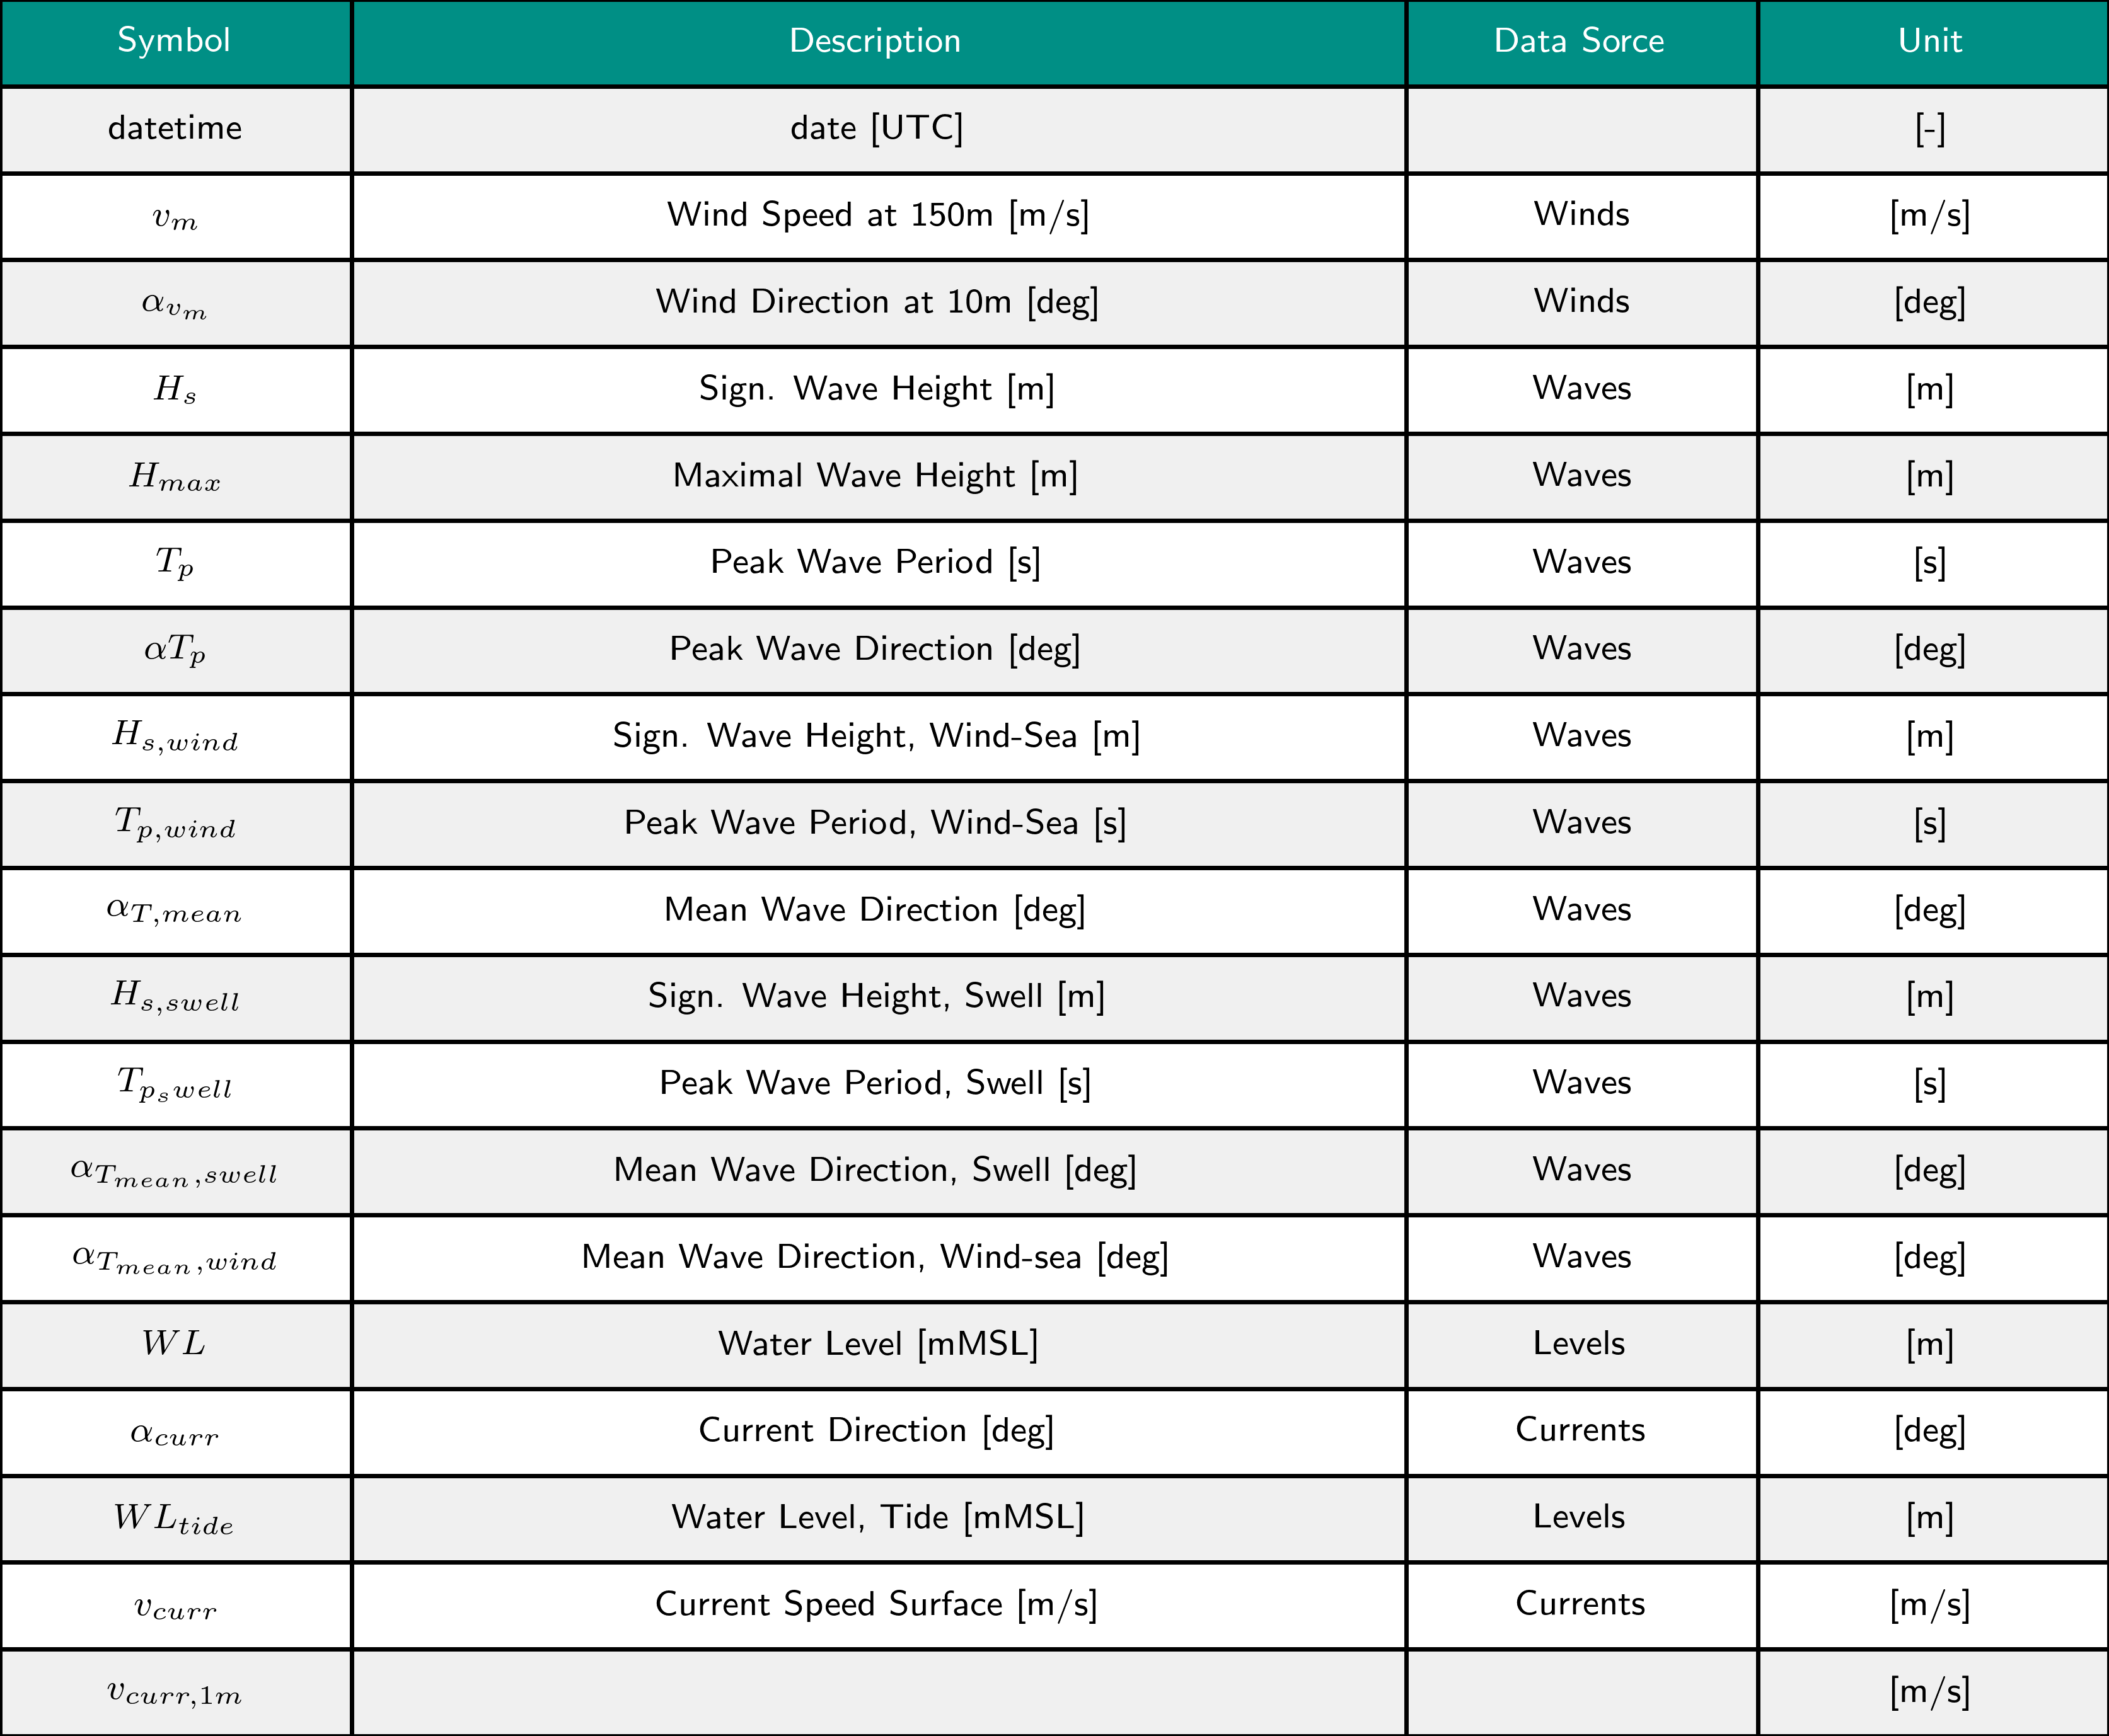
\includegraphics[width=1.0\textwidth ]{C:/Users/aaron.lange/Desktop/Projekte/Hindcast_Tool/HindTool/example_output/Sensor_names_page_1.png} 
 \captionsetup{type=table} 
\caption{ Sensor-names-page-1 } 
 \label{tab: Sensor_names_page_1 } 
\end{figure}

\clearpage 

\subsection{Sensor illustration}

\subsubsection{Sensor: Wind Speed at 150m [m/s]} 
\begin{figure}[H] 
 \centering 
 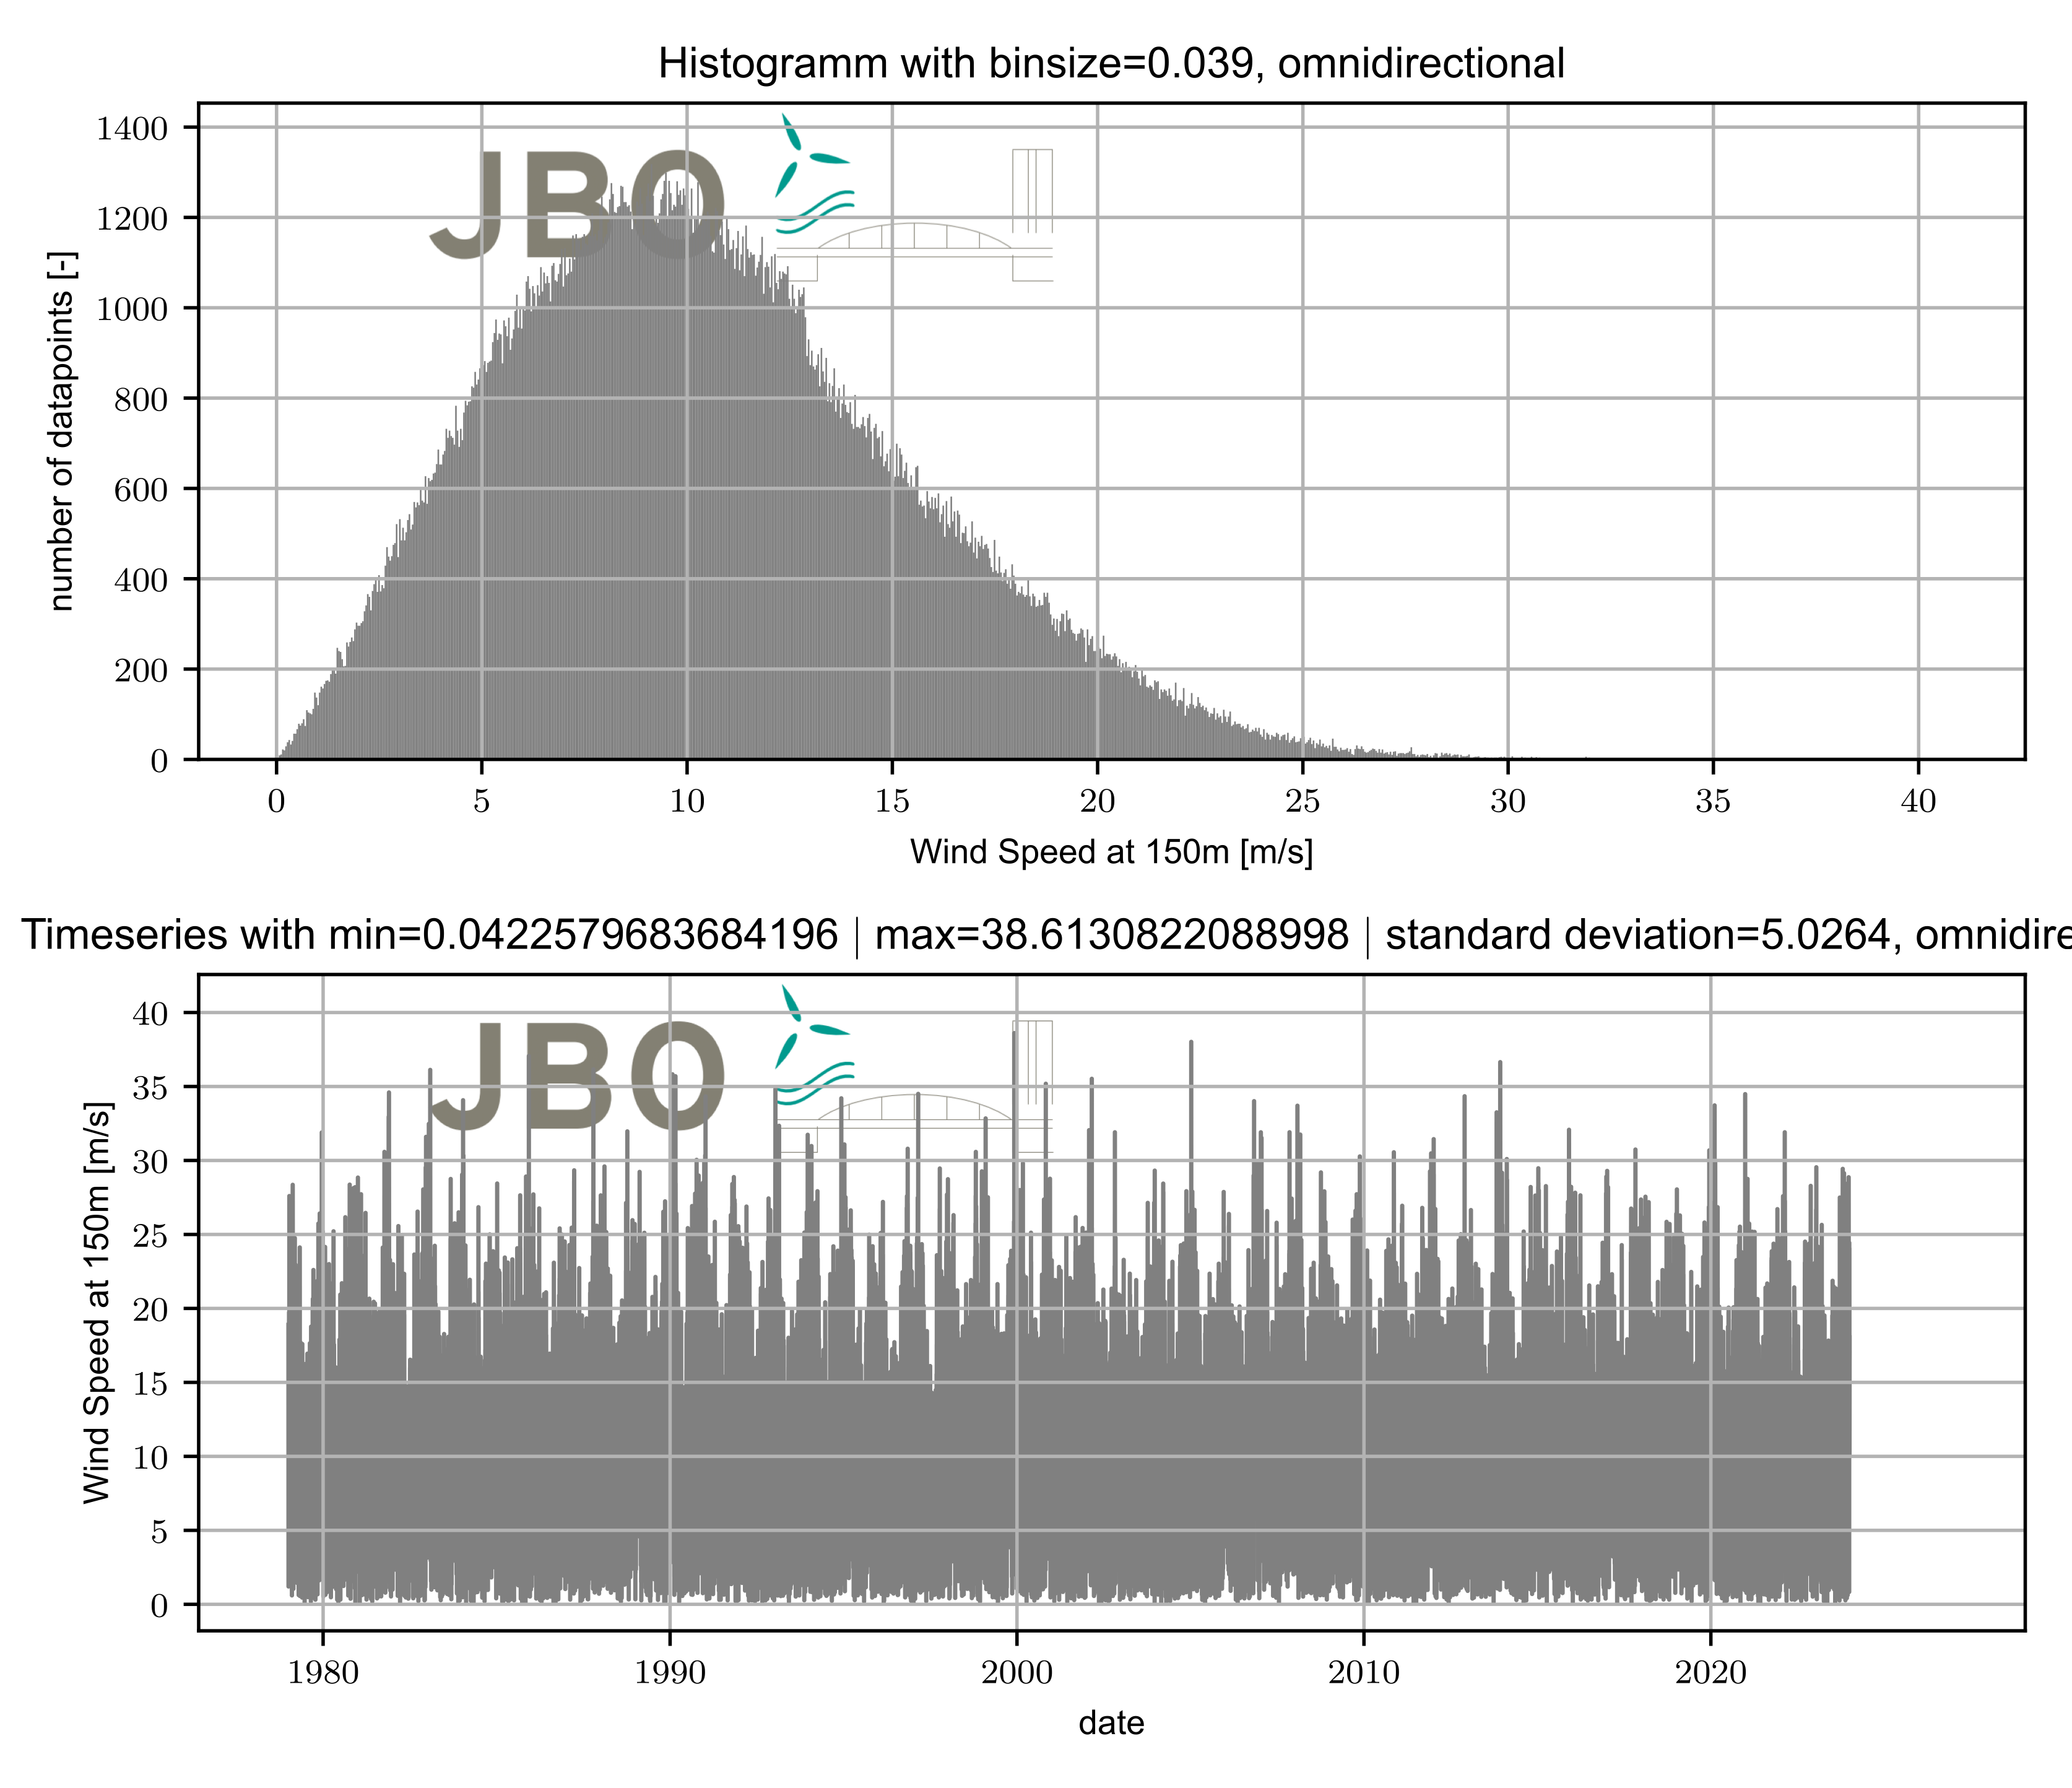
\includegraphics[width=1.0\textwidth]{C:/Users/aaron.lange/Desktop/Projekte/Hindcast_Tool/HindTool/example_output/SensorEval_v_m_page_1.png} 
 \caption{ Timeseries and Histogram of Sensor: Wind Speed at 150m [m/s] } 
 \label{fig: SensorEval_v_m_page_1 } 
\end{figure}
 \clearpage
\subsubsection{Sensor: Sign. Wave Height [m]} 
\begin{figure}[H] 
 \centering 
 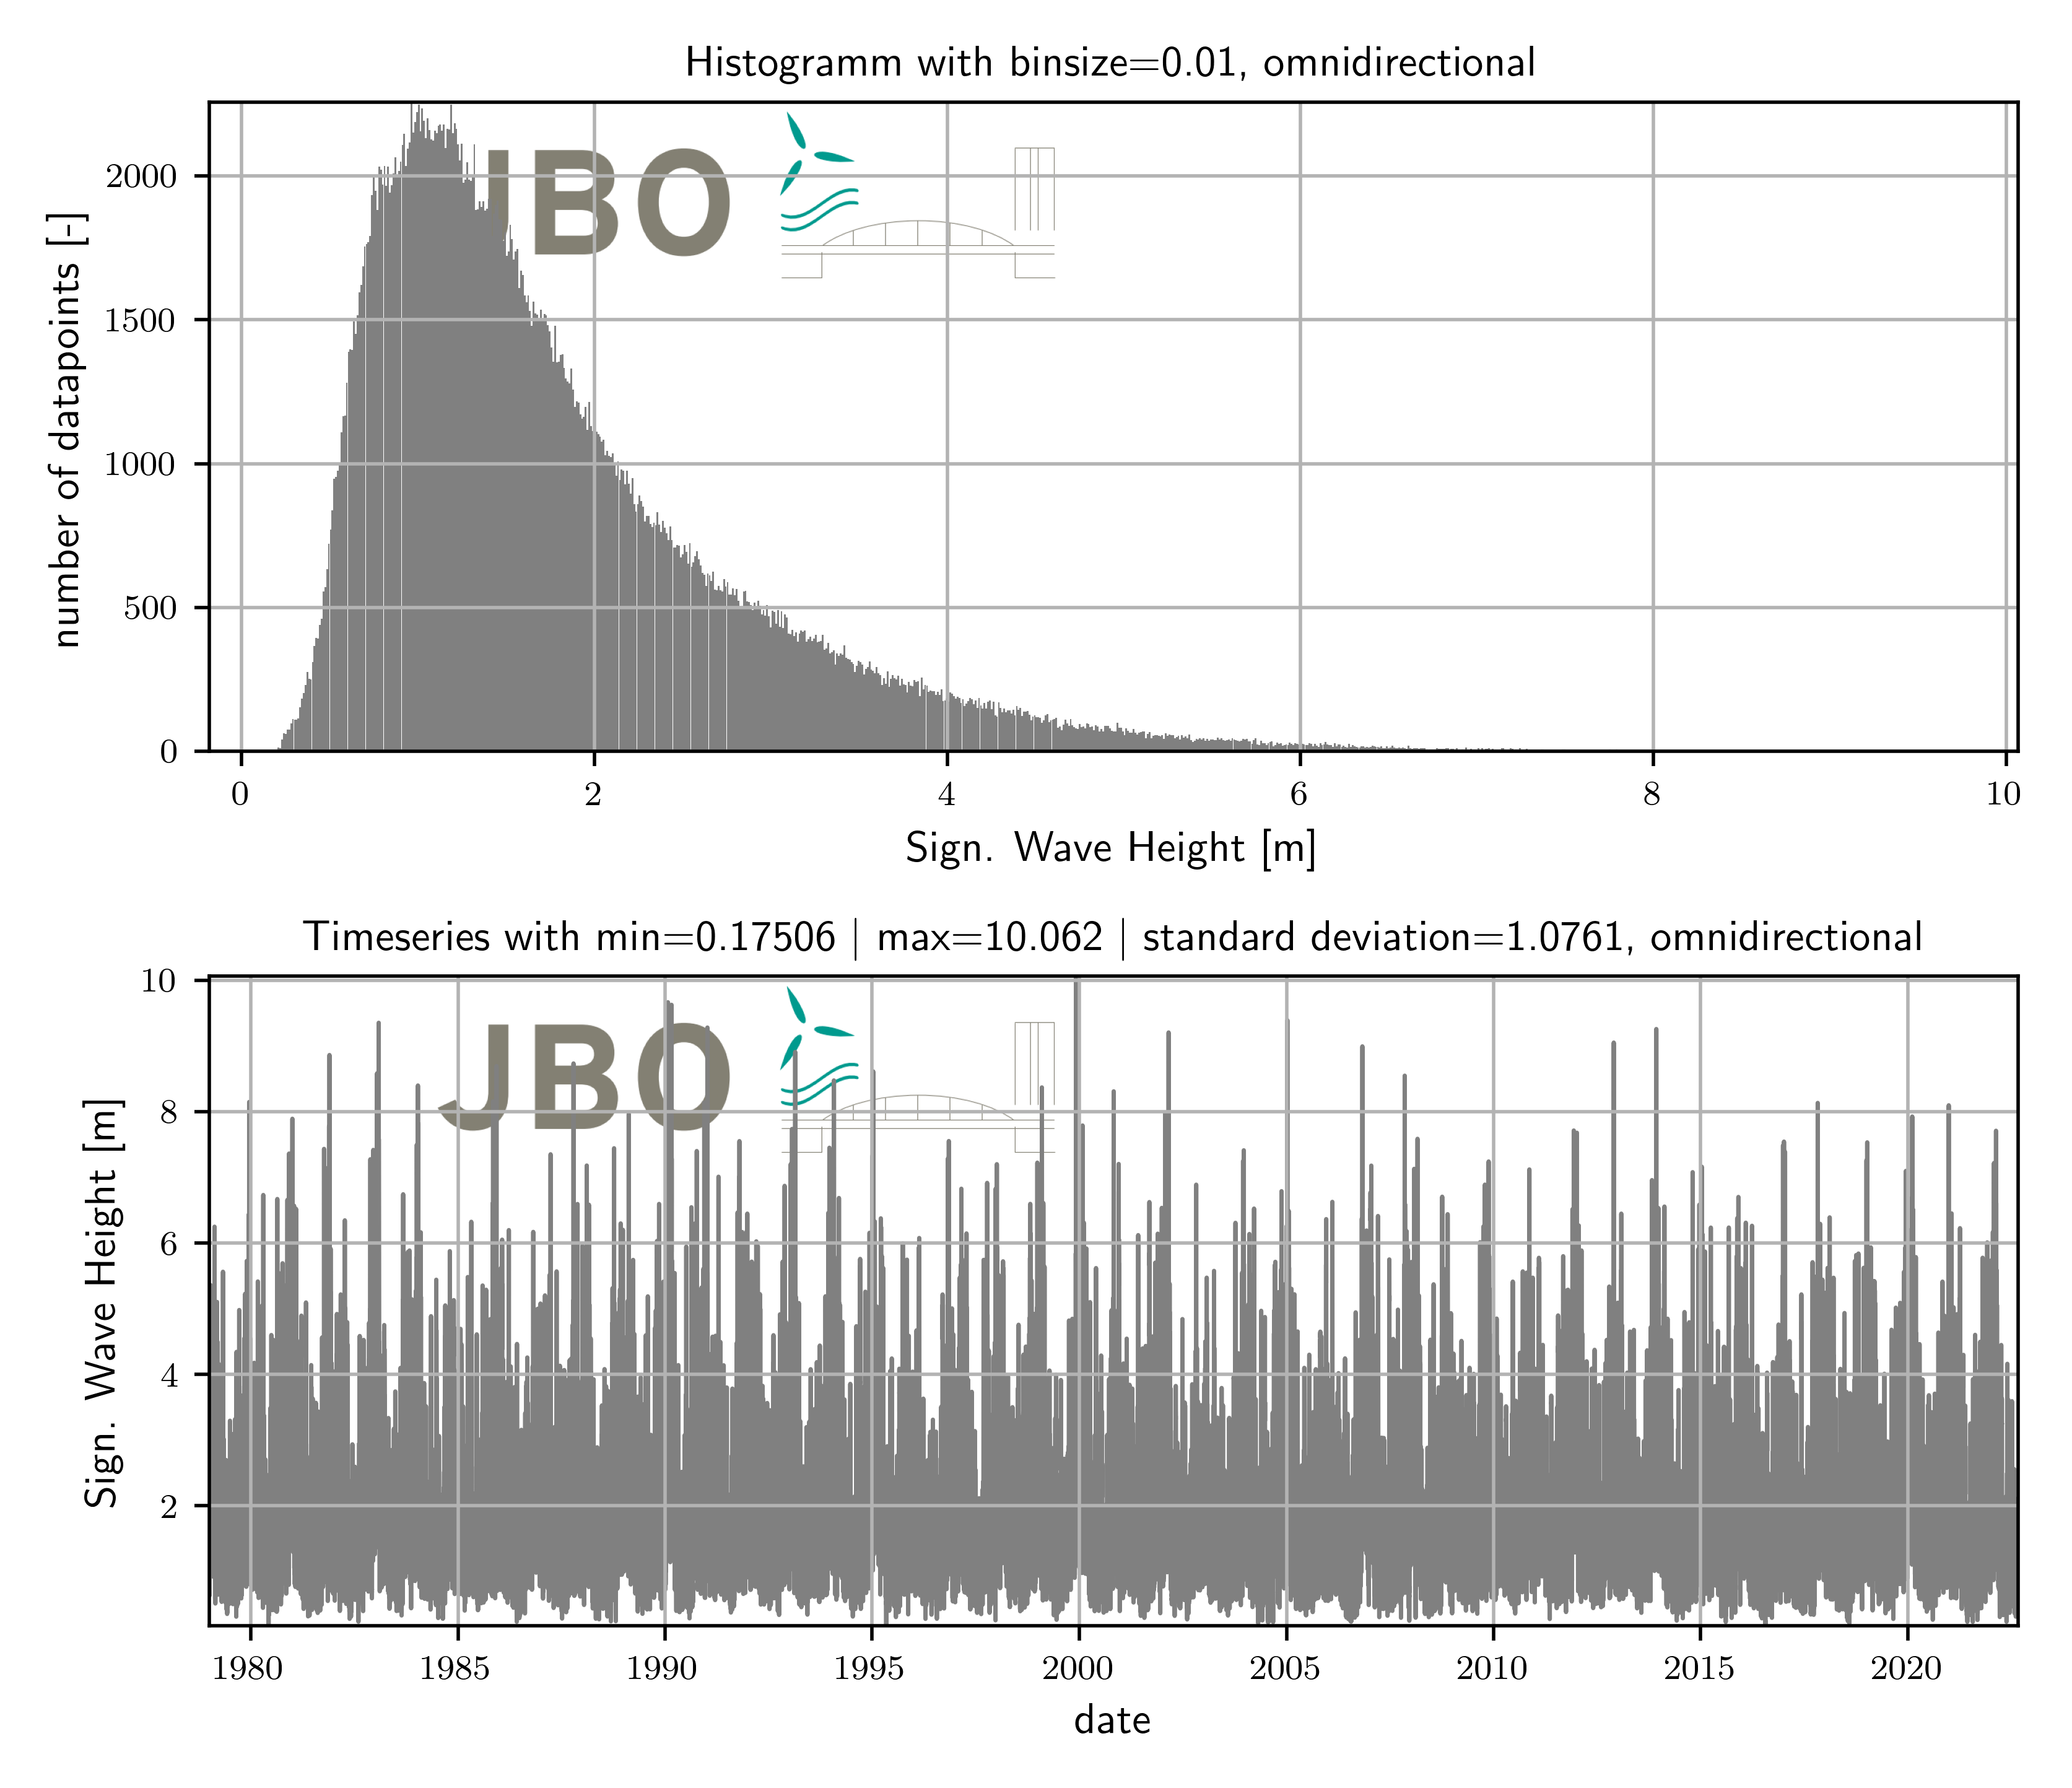
\includegraphics[width=1.0\textwidth]{C:/Users/aaron.lange/Desktop/Projekte/Hindcast_Tool/HindTool/example_output/SensorEval_H_s_page_1.png} 
 \caption{ Timeseries and Histogram of Sensor: Sign. Wave Height [m] } 
 \label{fig: SensorEval_H_s_page_1 } 
\end{figure}
 \clearpage
\subsubsection{Sensor: Maximal Wave Height [m]} 
\begin{figure}[H] 
 \centering 
 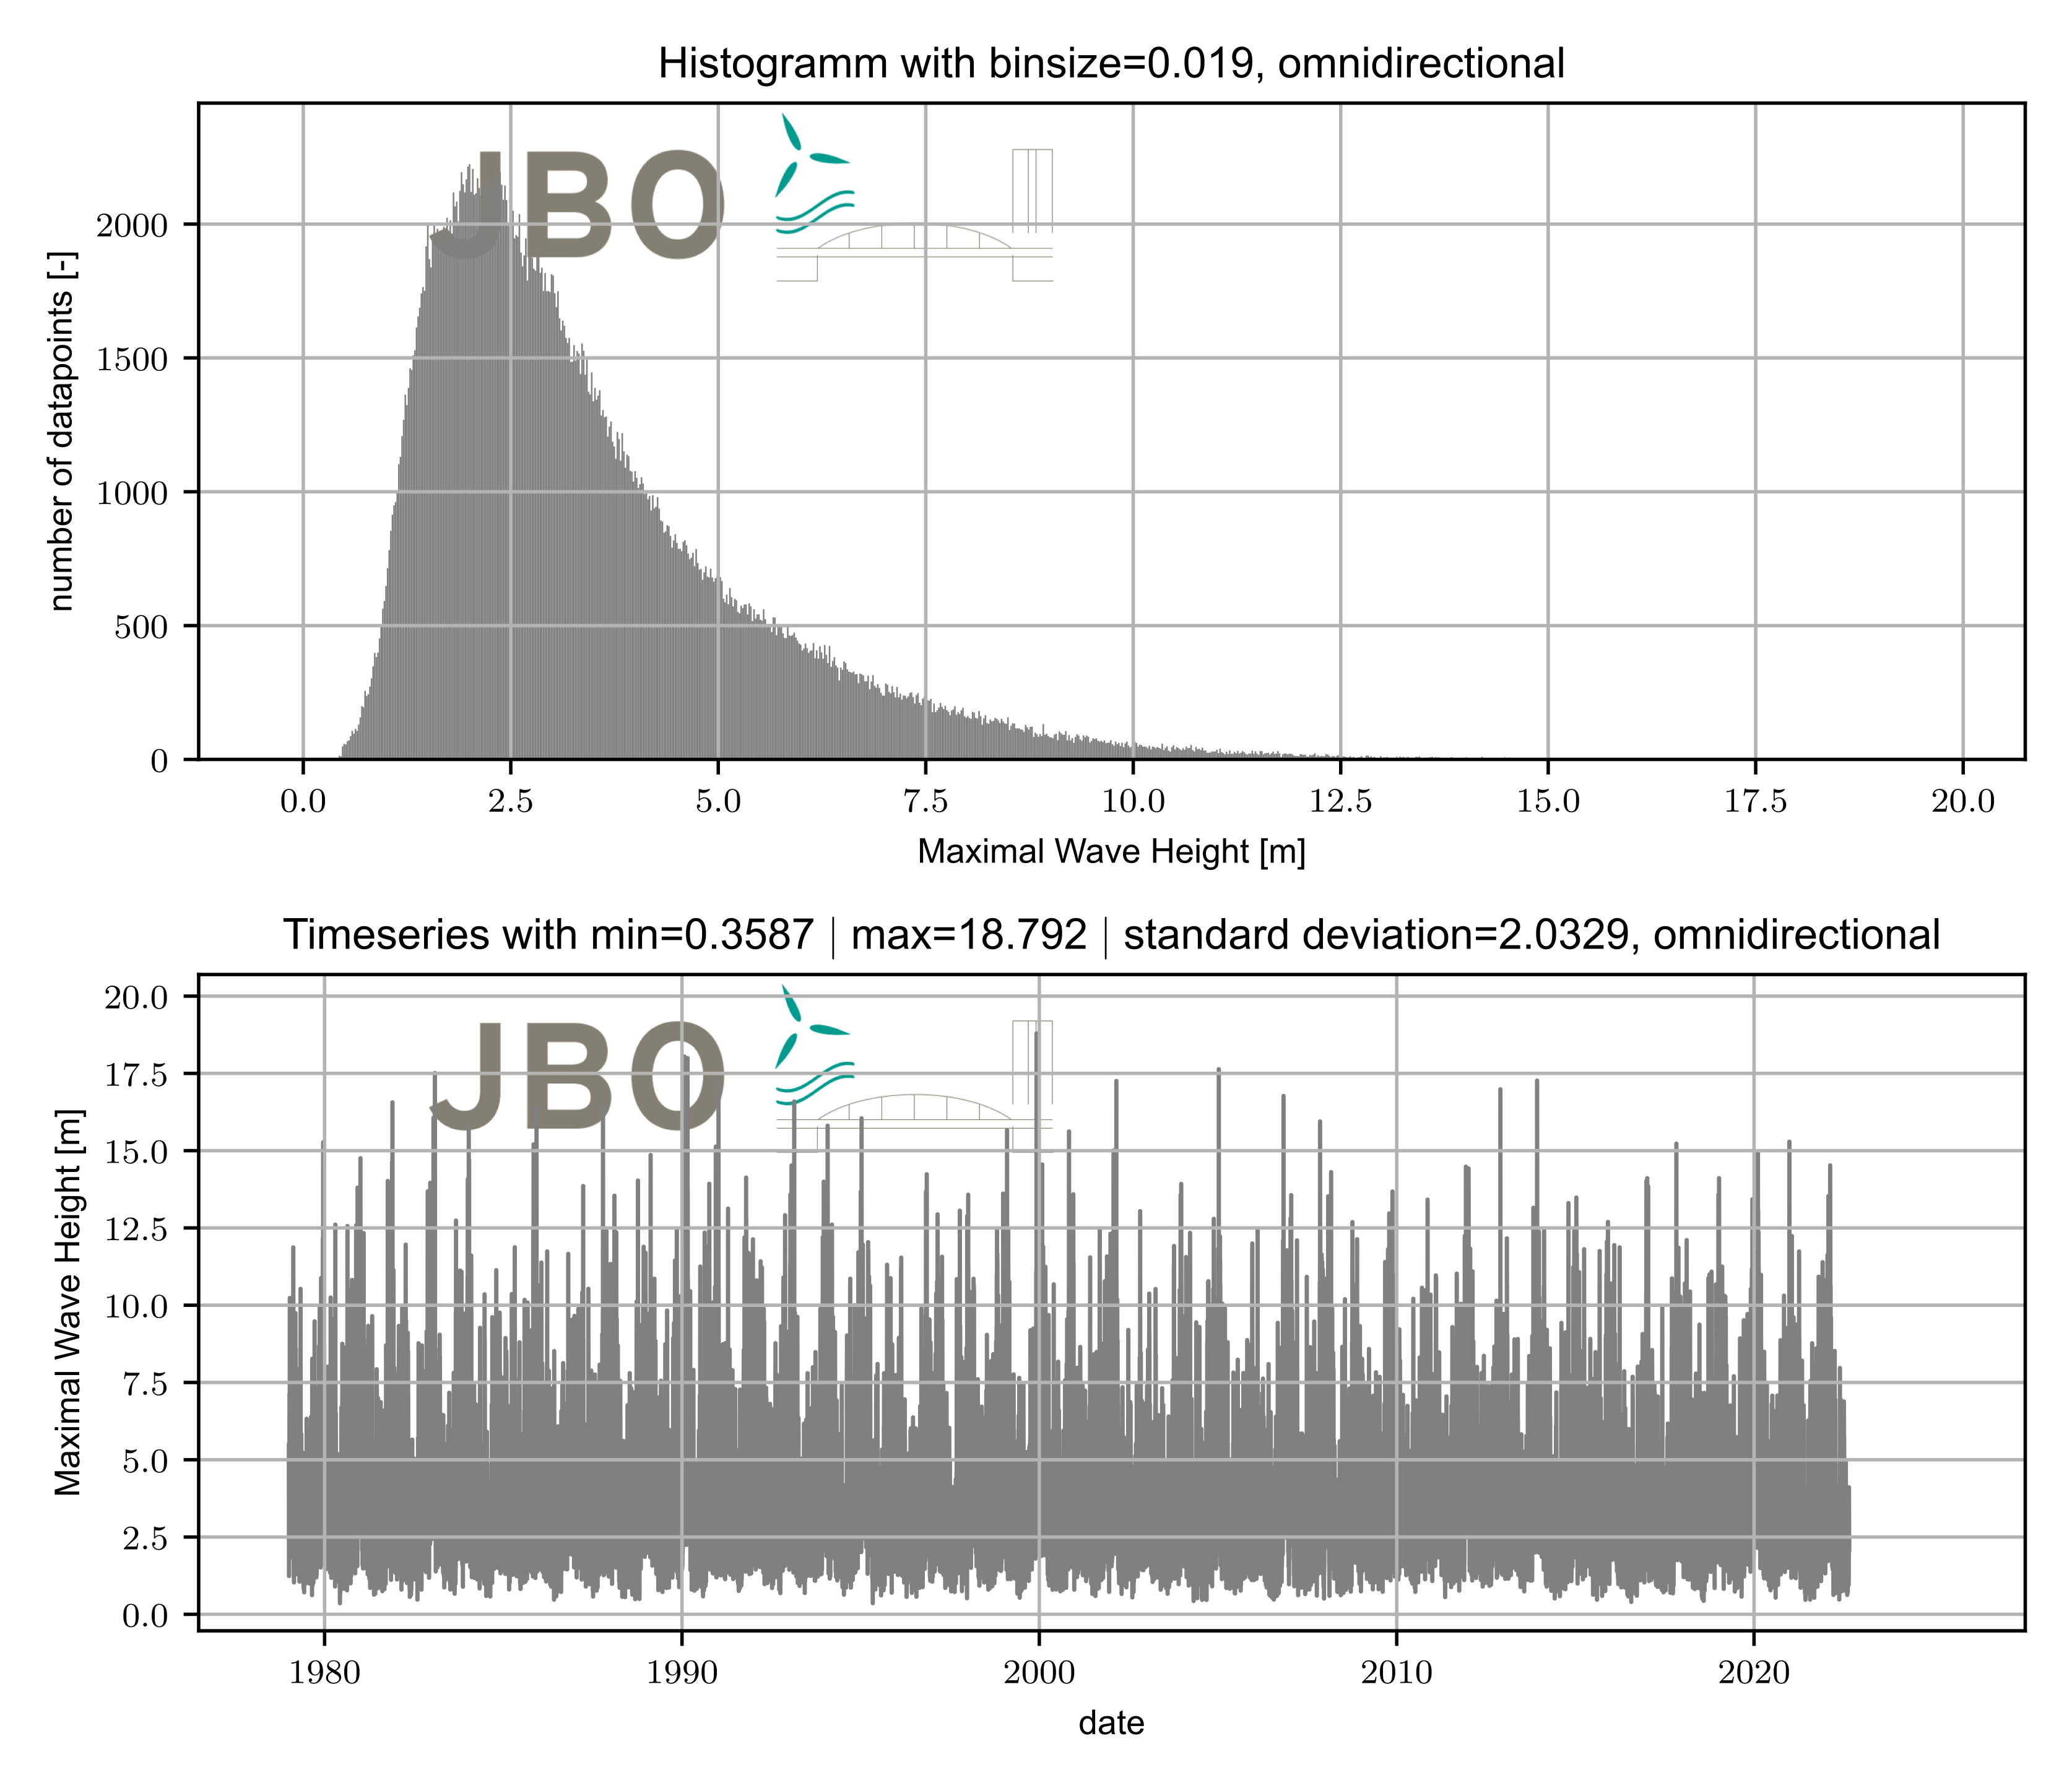
\includegraphics[width=1.0\textwidth]{C:/Users/aaron.lange/Desktop/Projekte/Hindcast_Tool/HindTool/example_output/SensorEval_H_max_page_1.png} 
 \caption{ Timeseries and Histogram of Sensor: Maximal Wave Height [m] } 
 \label{fig: SensorEval_H_max_page_1 } 
\end{figure}
 \clearpage
\subsubsection{Sensor: Peak Wave Period [s]} 
\begin{figure}[H] 
 \centering 
 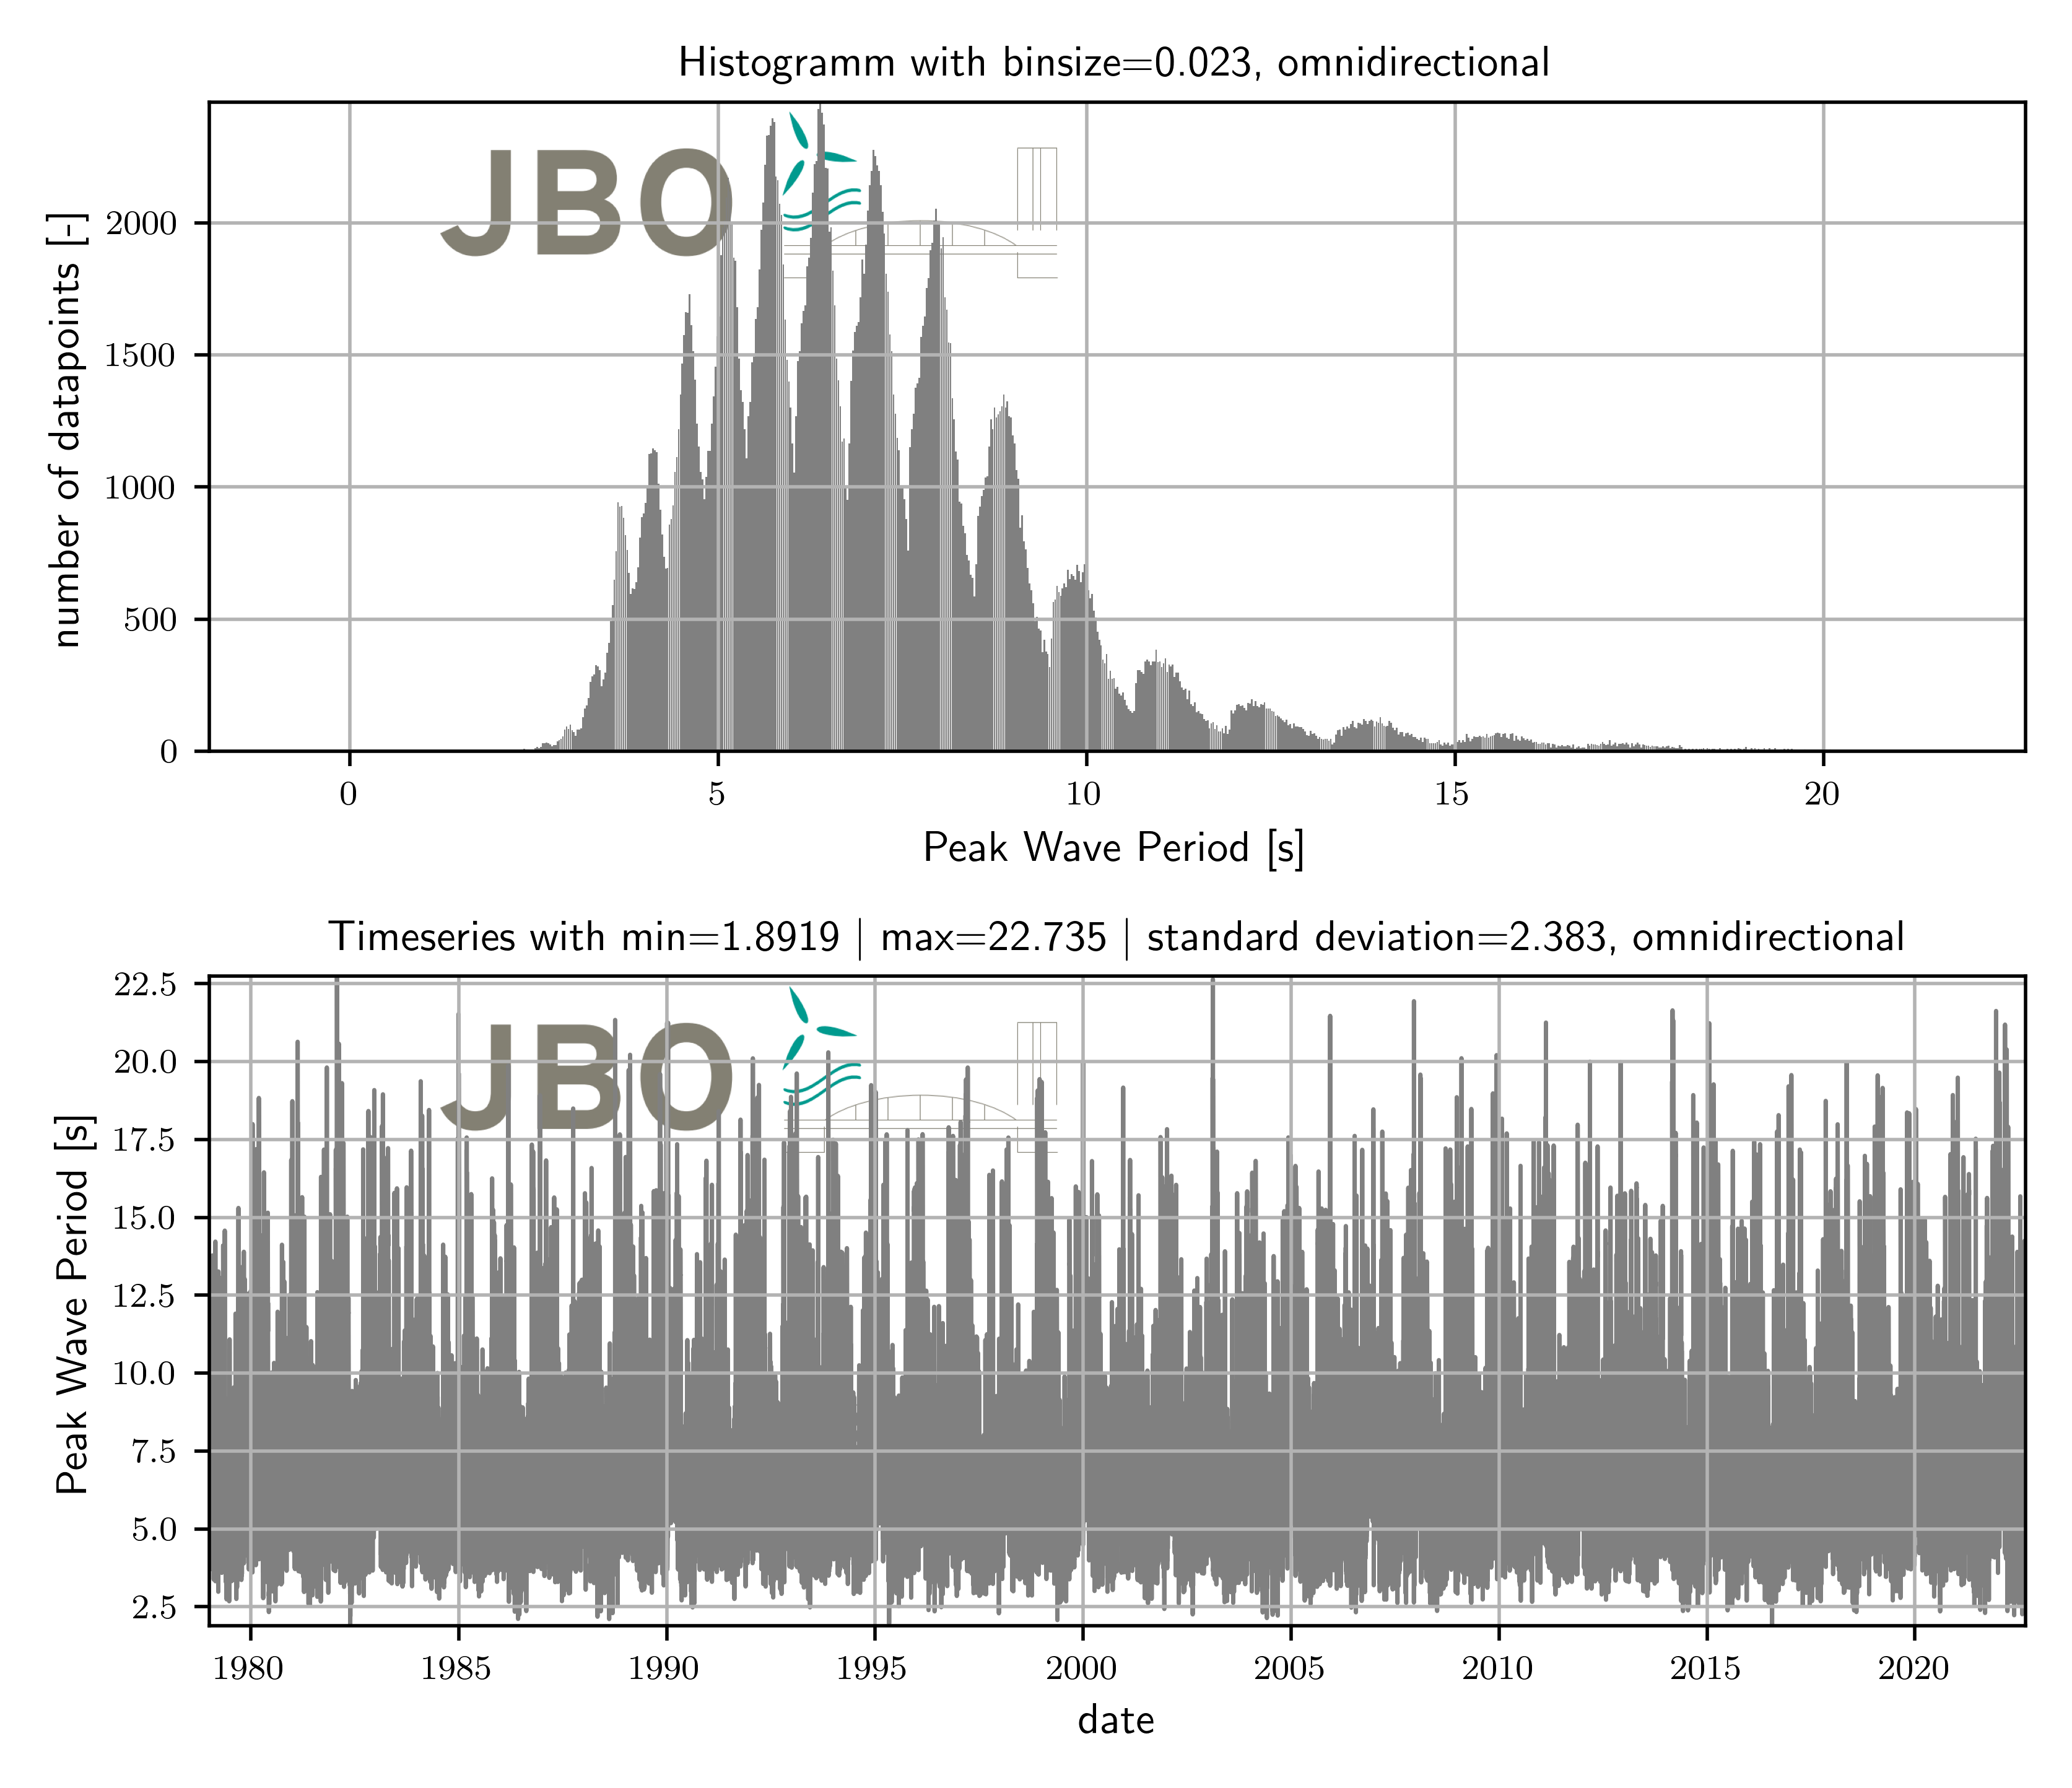
\includegraphics[width=1.0\textwidth]{C:/Users/aaron.lange/Desktop/Projekte/Hindcast_Tool/HindTool/example_output/SensorEval_T_p_page_1.png} 
 \caption{ Timeseries and Histogram of Sensor: Peak Wave Period [s] } 
 \label{fig: SensorEval_T_p_page_1 } 
\end{figure}
 \clearpage
\subsubsection{Sensor: Sign. Wave Height, Wind-Sea [m]} 
\begin{figure}[H] 
 \centering 
 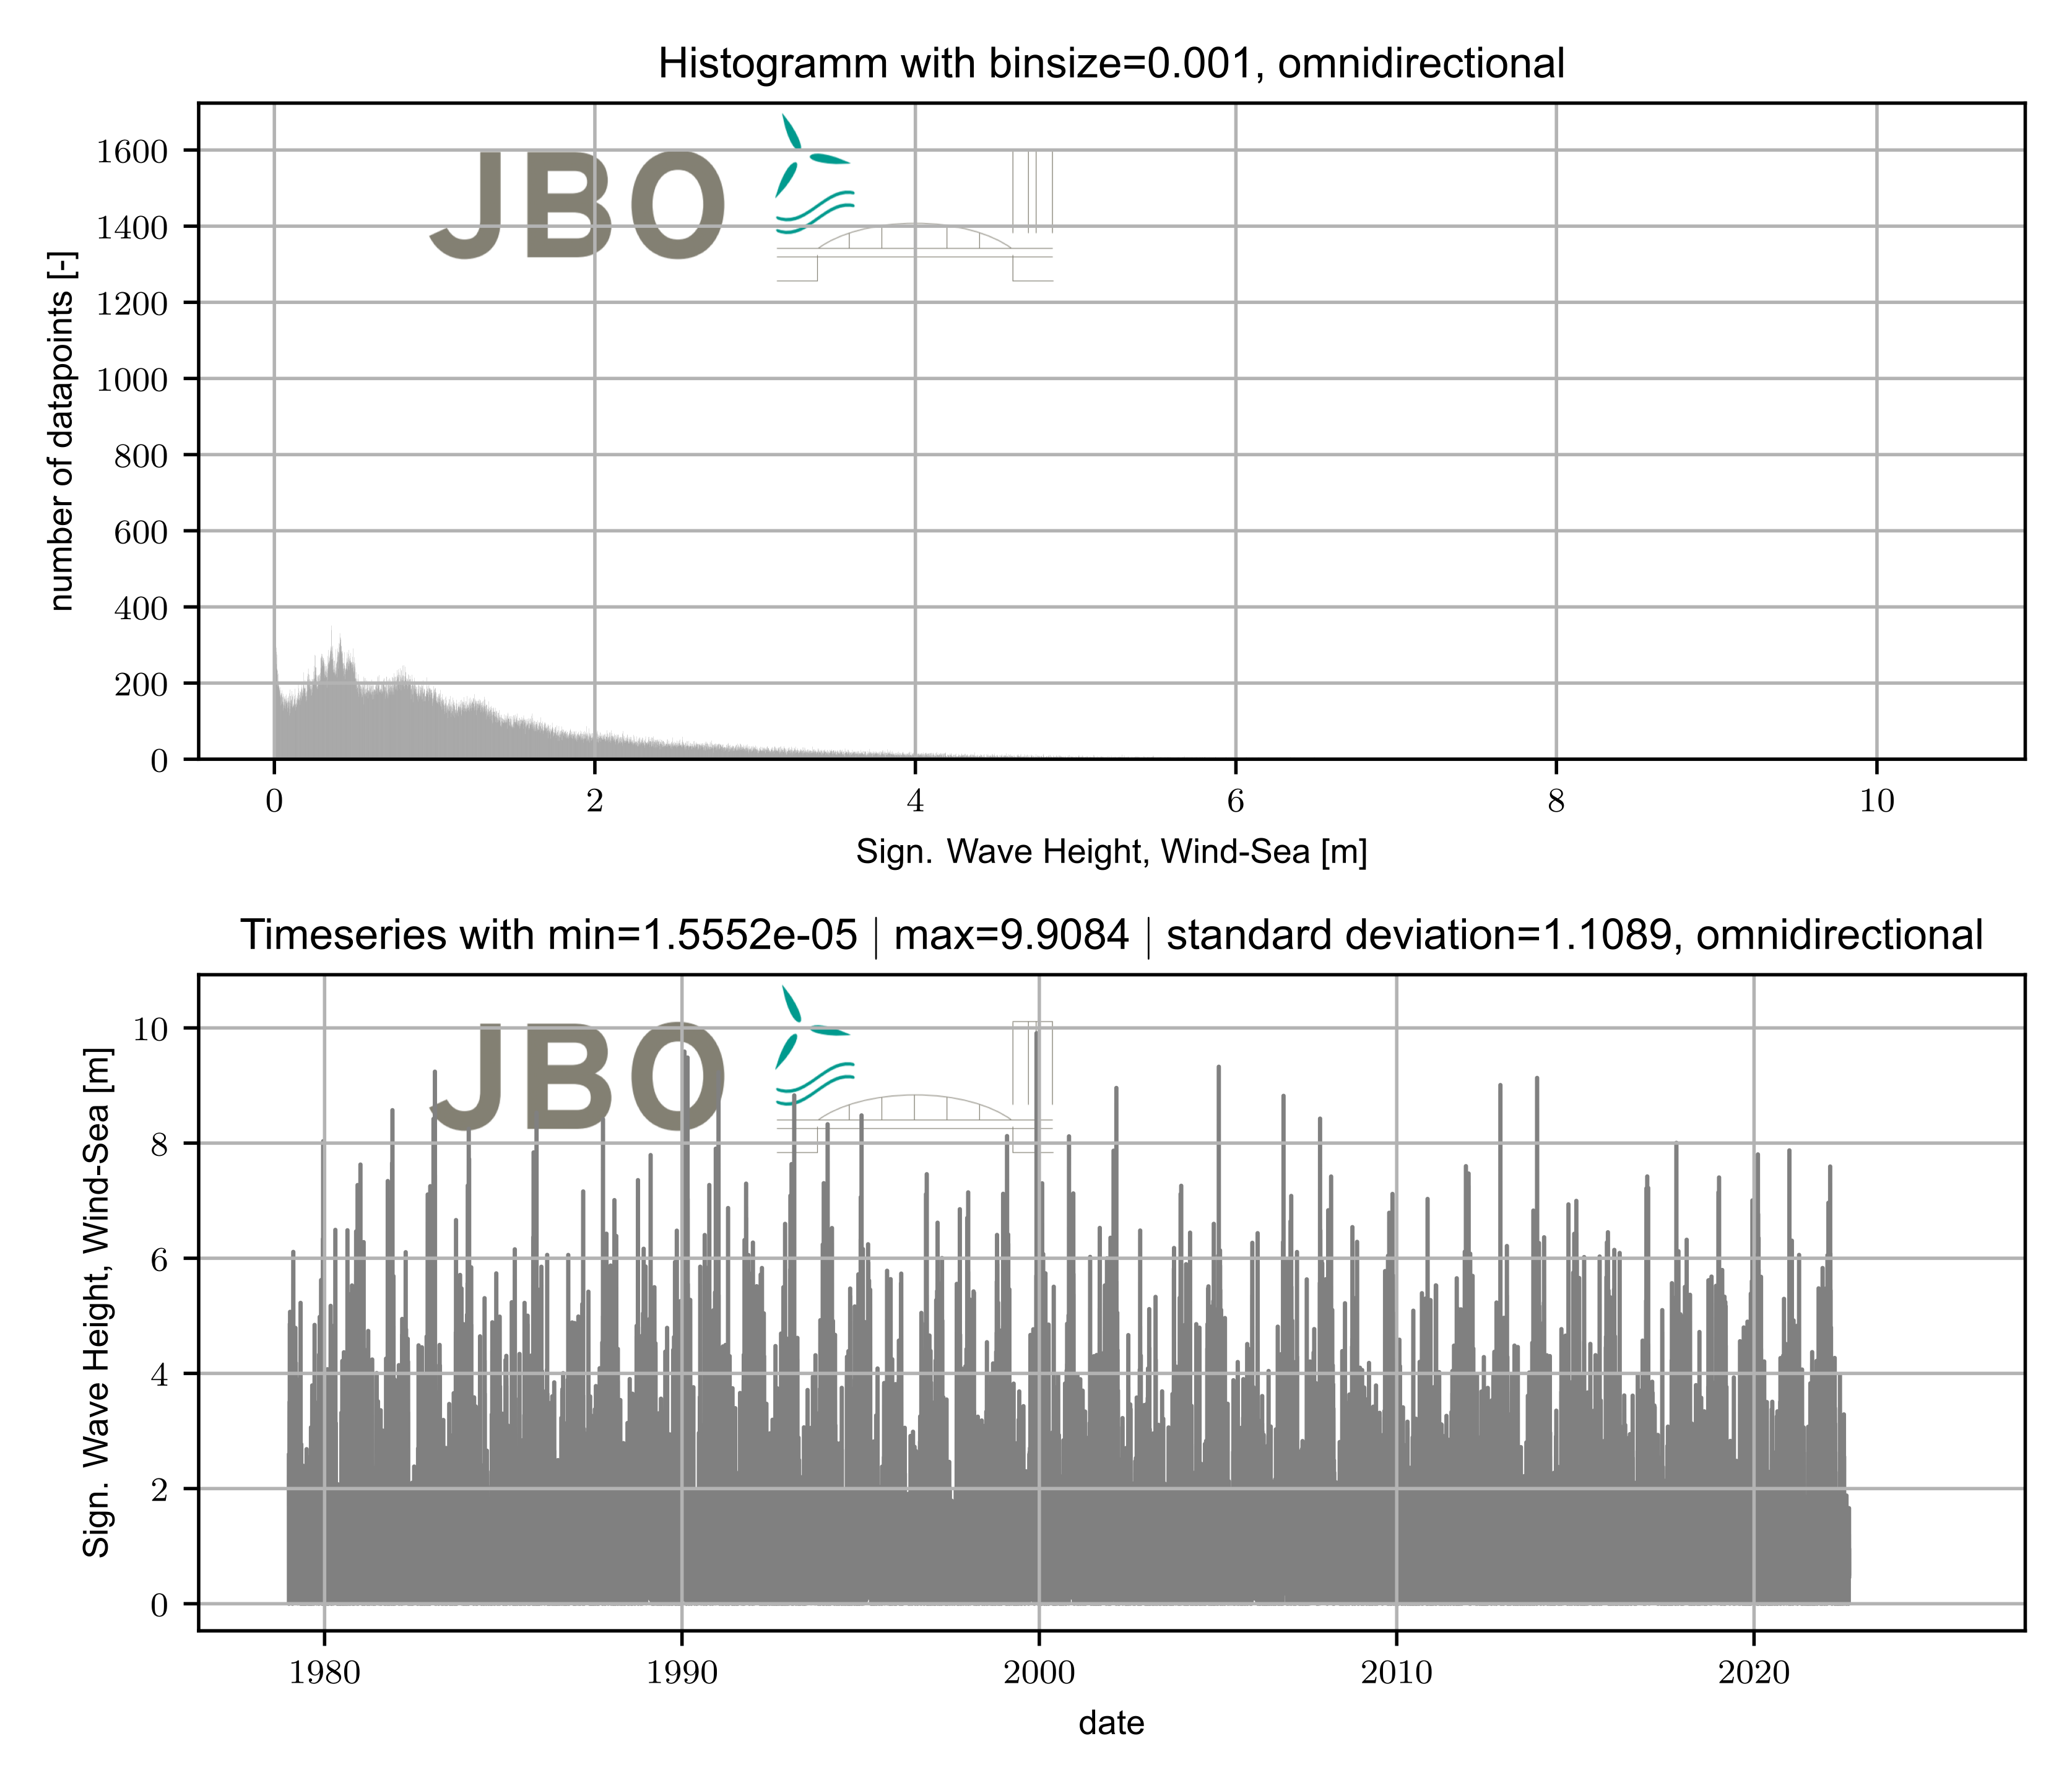
\includegraphics[width=1.0\textwidth]{C:/Users/aaron.lange/Desktop/Projekte/Hindcast_Tool/HindTool/example_output/SensorEval_H_s_wind_page_1.png} 
 \caption{ Timeseries and Histogram of Sensor: Sign. Wave Height, Wind-Sea [m] } 
 \label{fig: SensorEval_H_s_wind_page_1 } 
\end{figure}
 \clearpage
\subsubsection{Sensor: Peak Wave Period, Wind-Sea [s]} 
\begin{figure}[H] 
 \centering 
 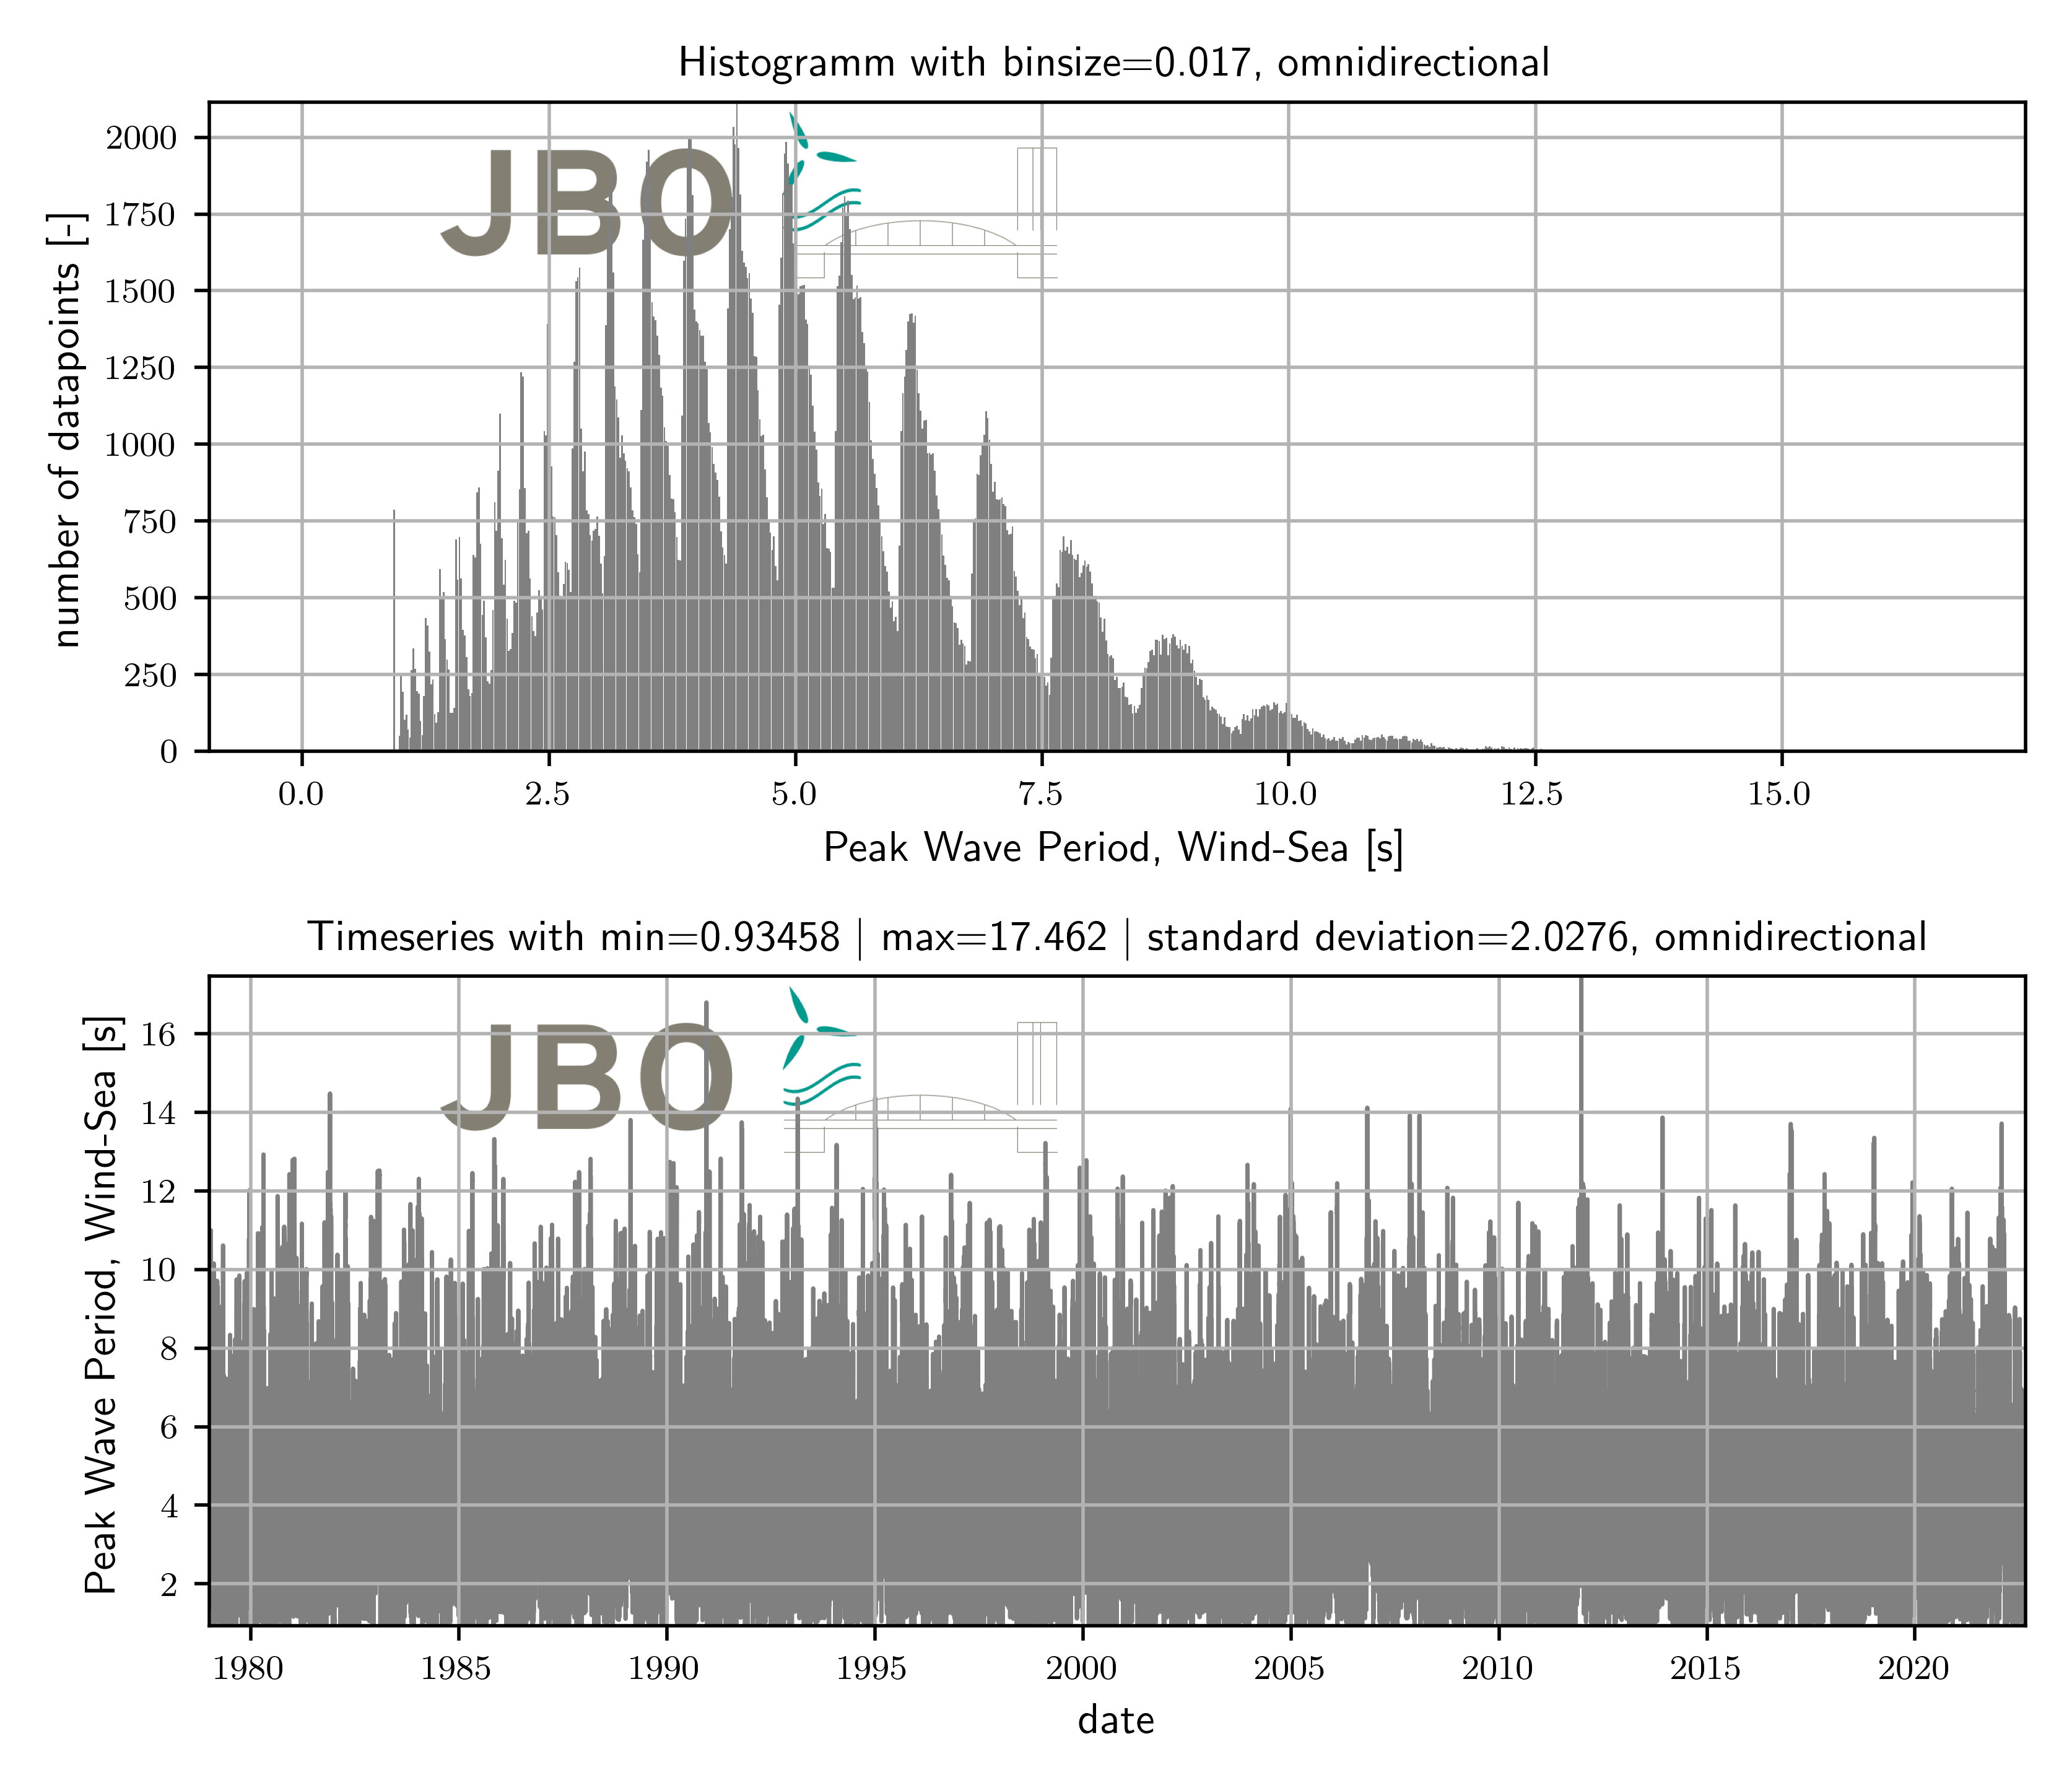
\includegraphics[width=1.0\textwidth]{C:/Users/aaron.lange/Desktop/Projekte/Hindcast_Tool/HindTool/example_output/SensorEval_T_p_wind_page_1.png} 
 \caption{ Timeseries and Histogram of Sensor: Peak Wave Period, Wind-Sea [s] } 
 \label{fig: SensorEval_T_p_wind_page_1 } 
\end{figure}
 \clearpage
\subsubsection{Sensor: Sign. Wave Height, Swell [m]} 
\begin{figure}[H] 
 \centering 
 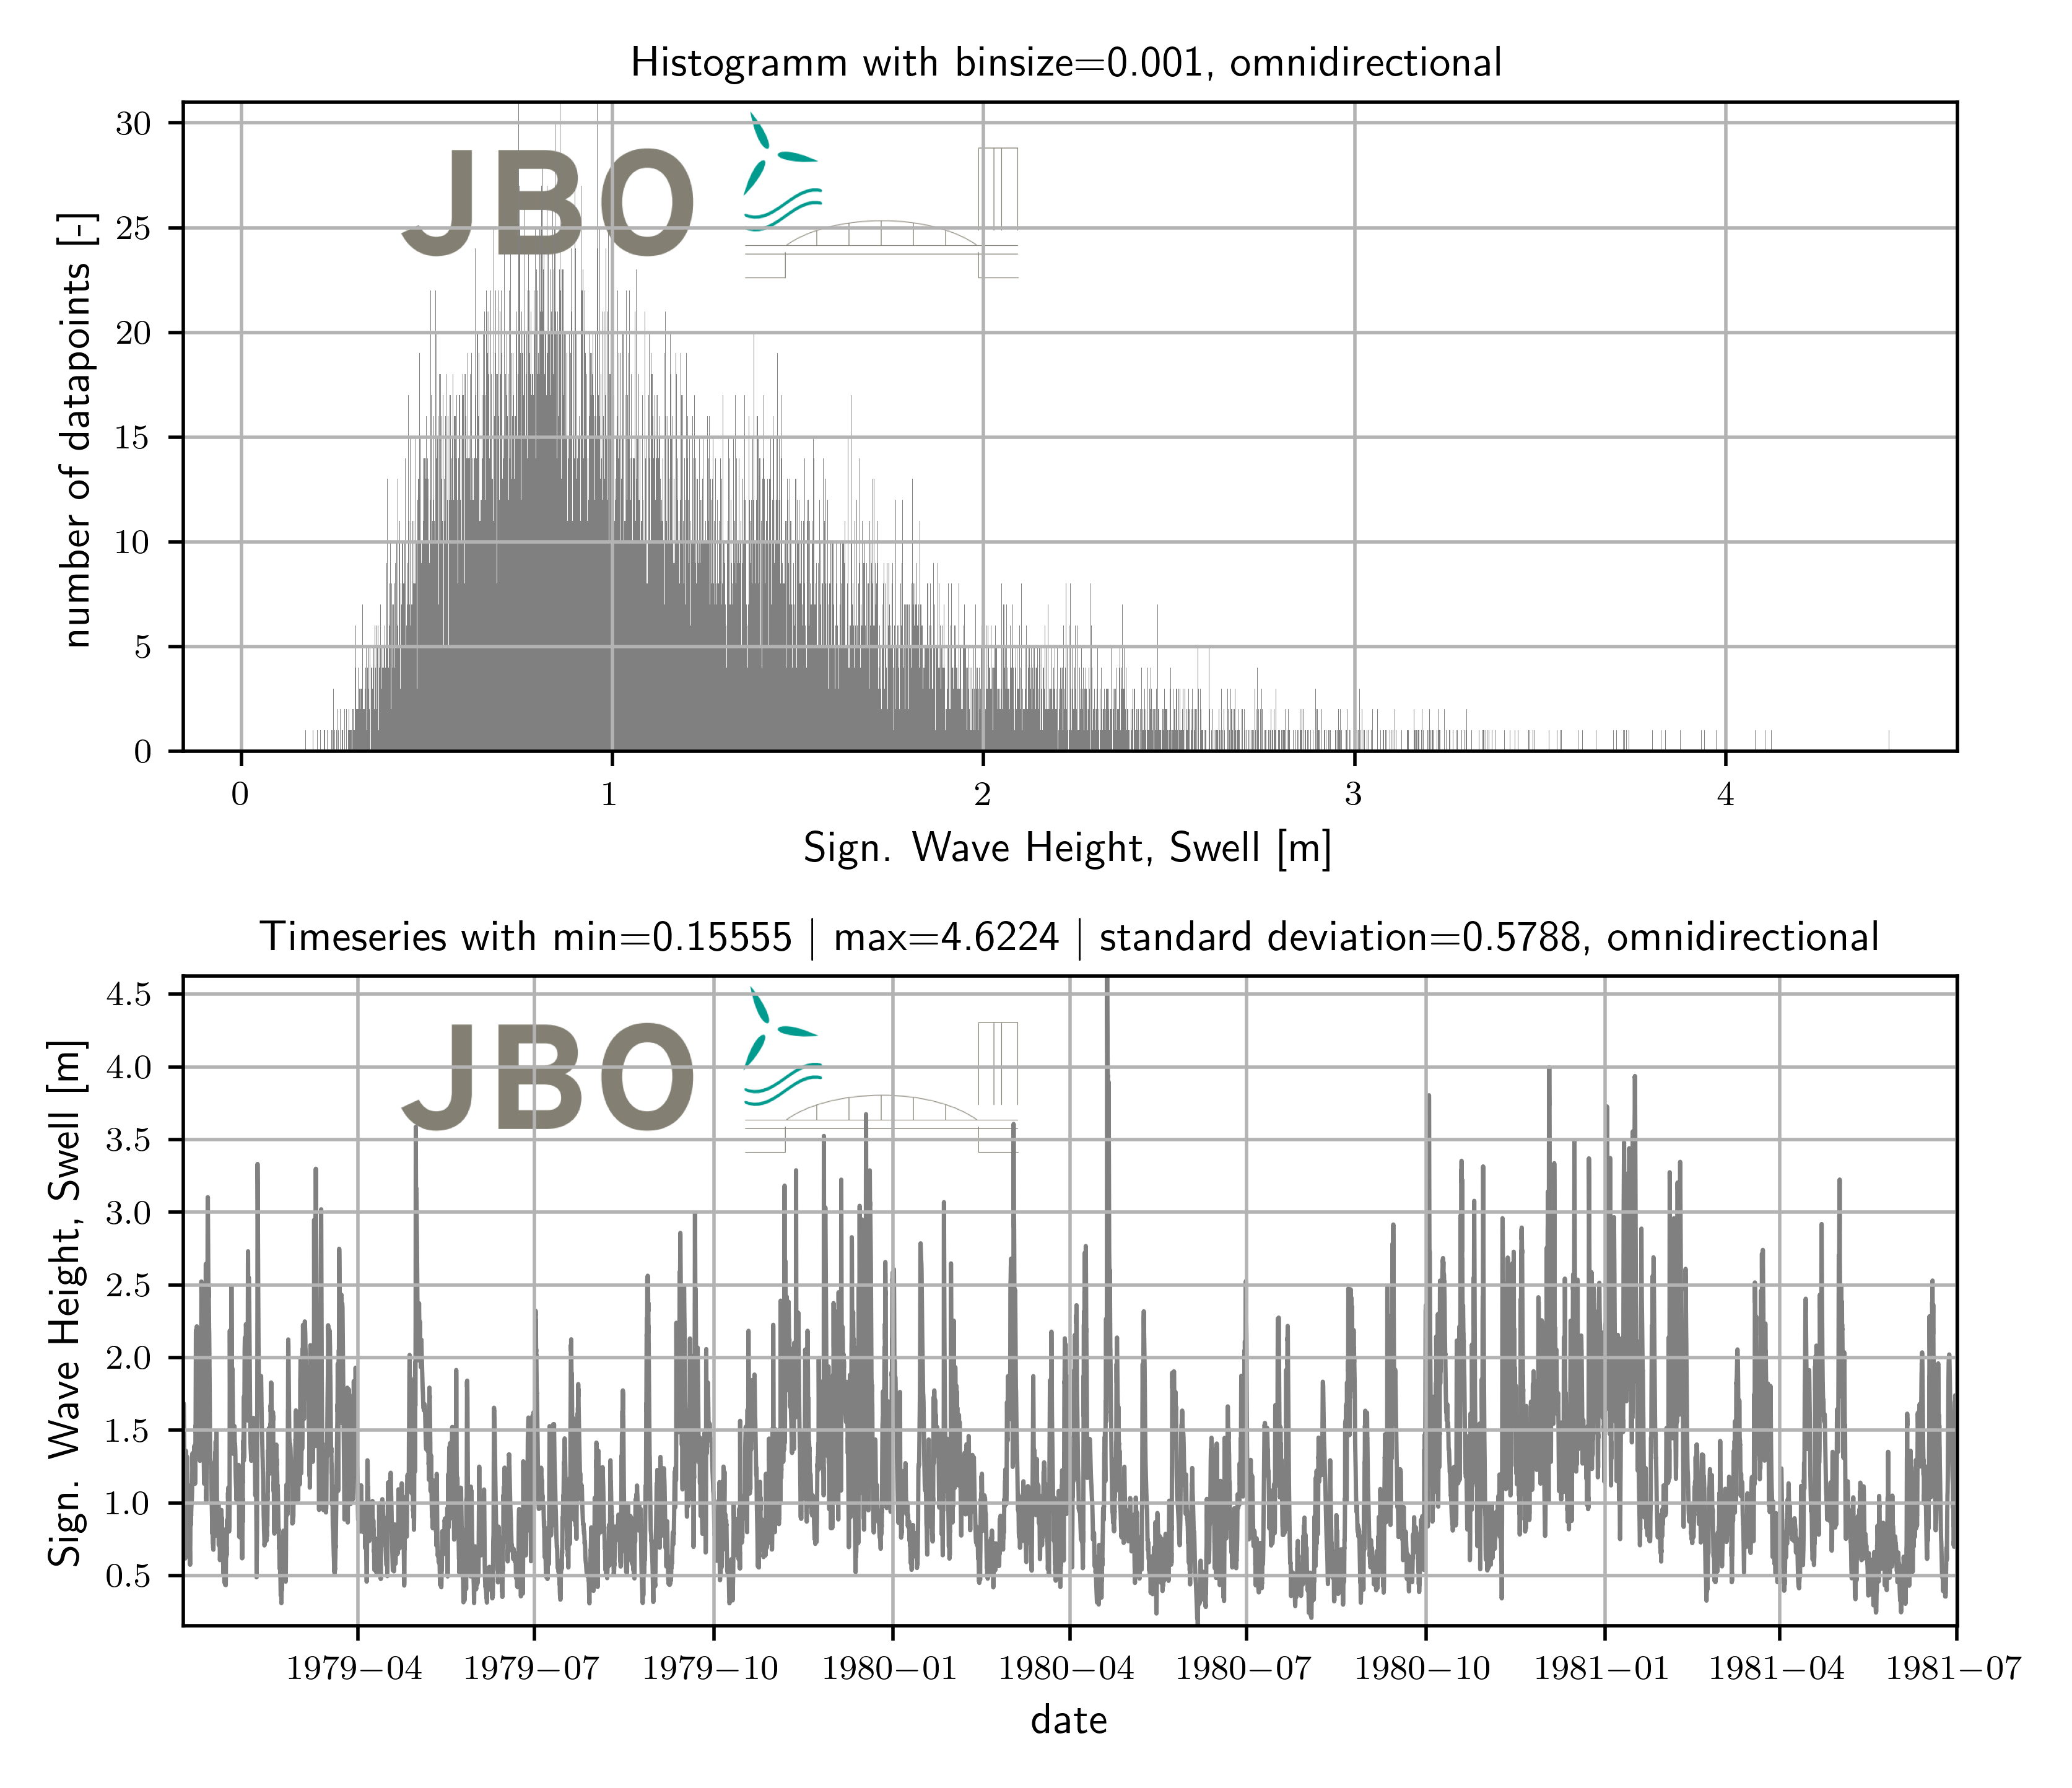
\includegraphics[width=1.0\textwidth]{C:/Users/aaron.lange/Desktop/Projekte/Hindcast_Tool/HindTool/example_output/SensorEval_H_s_swell_page_1.png} 
 \caption{ Timeseries and Histogram of Sensor: Sign. Wave Height, Swell [m] } 
 \label{fig: SensorEval_H_s_swell_page_1 } 
\end{figure}
 \clearpage
\subsubsection{Sensor: Peak Wave Period, Swell [s]} 
\begin{figure}[H] 
 \centering 
 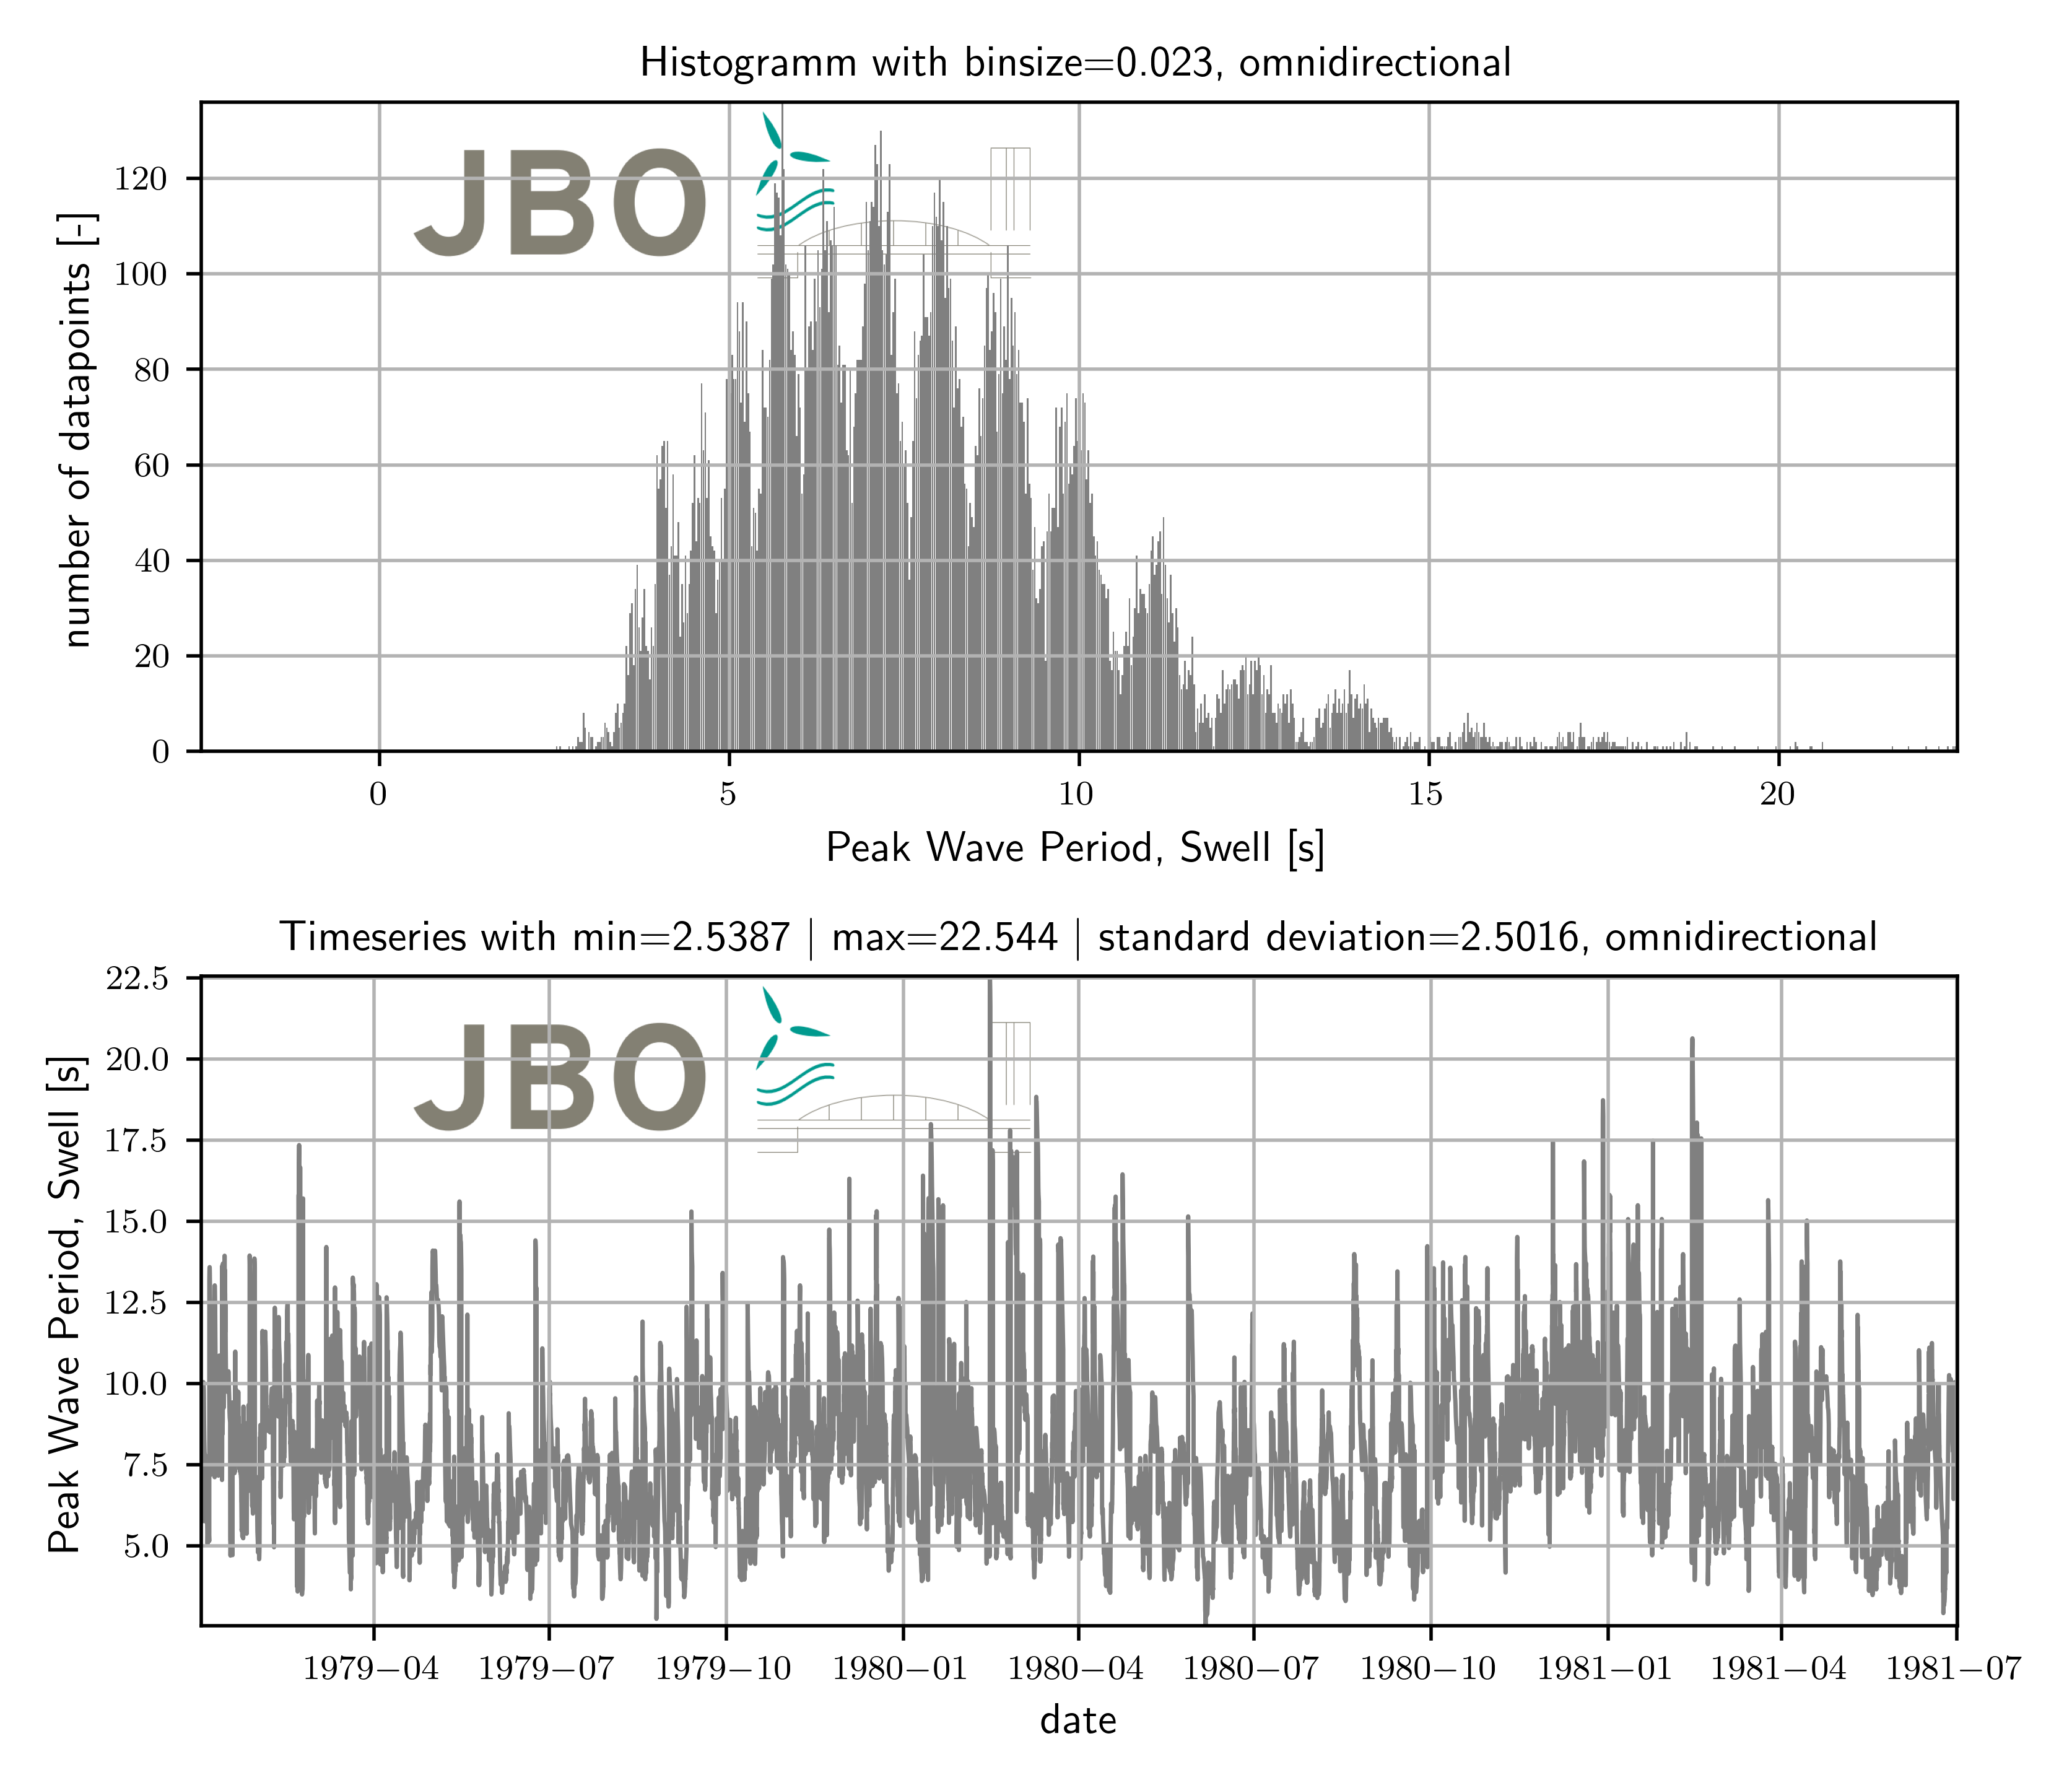
\includegraphics[width=1.0\textwidth]{C:/Users/aaron.lange/Desktop/Projekte/Hindcast_Tool/HindTool/example_output/SensorEval_T_p_swell_page_1.png} 
 \caption{ Timeseries and Histogram of Sensor: Peak Wave Period, Swell [s] } 
 \label{fig: SensorEval_T_p_swell_page_1 } 
\end{figure}
 \clearpage
\subsubsection{Sensor: Water Level [mMSL]} 
\begin{figure}[H] 
 \centering 
 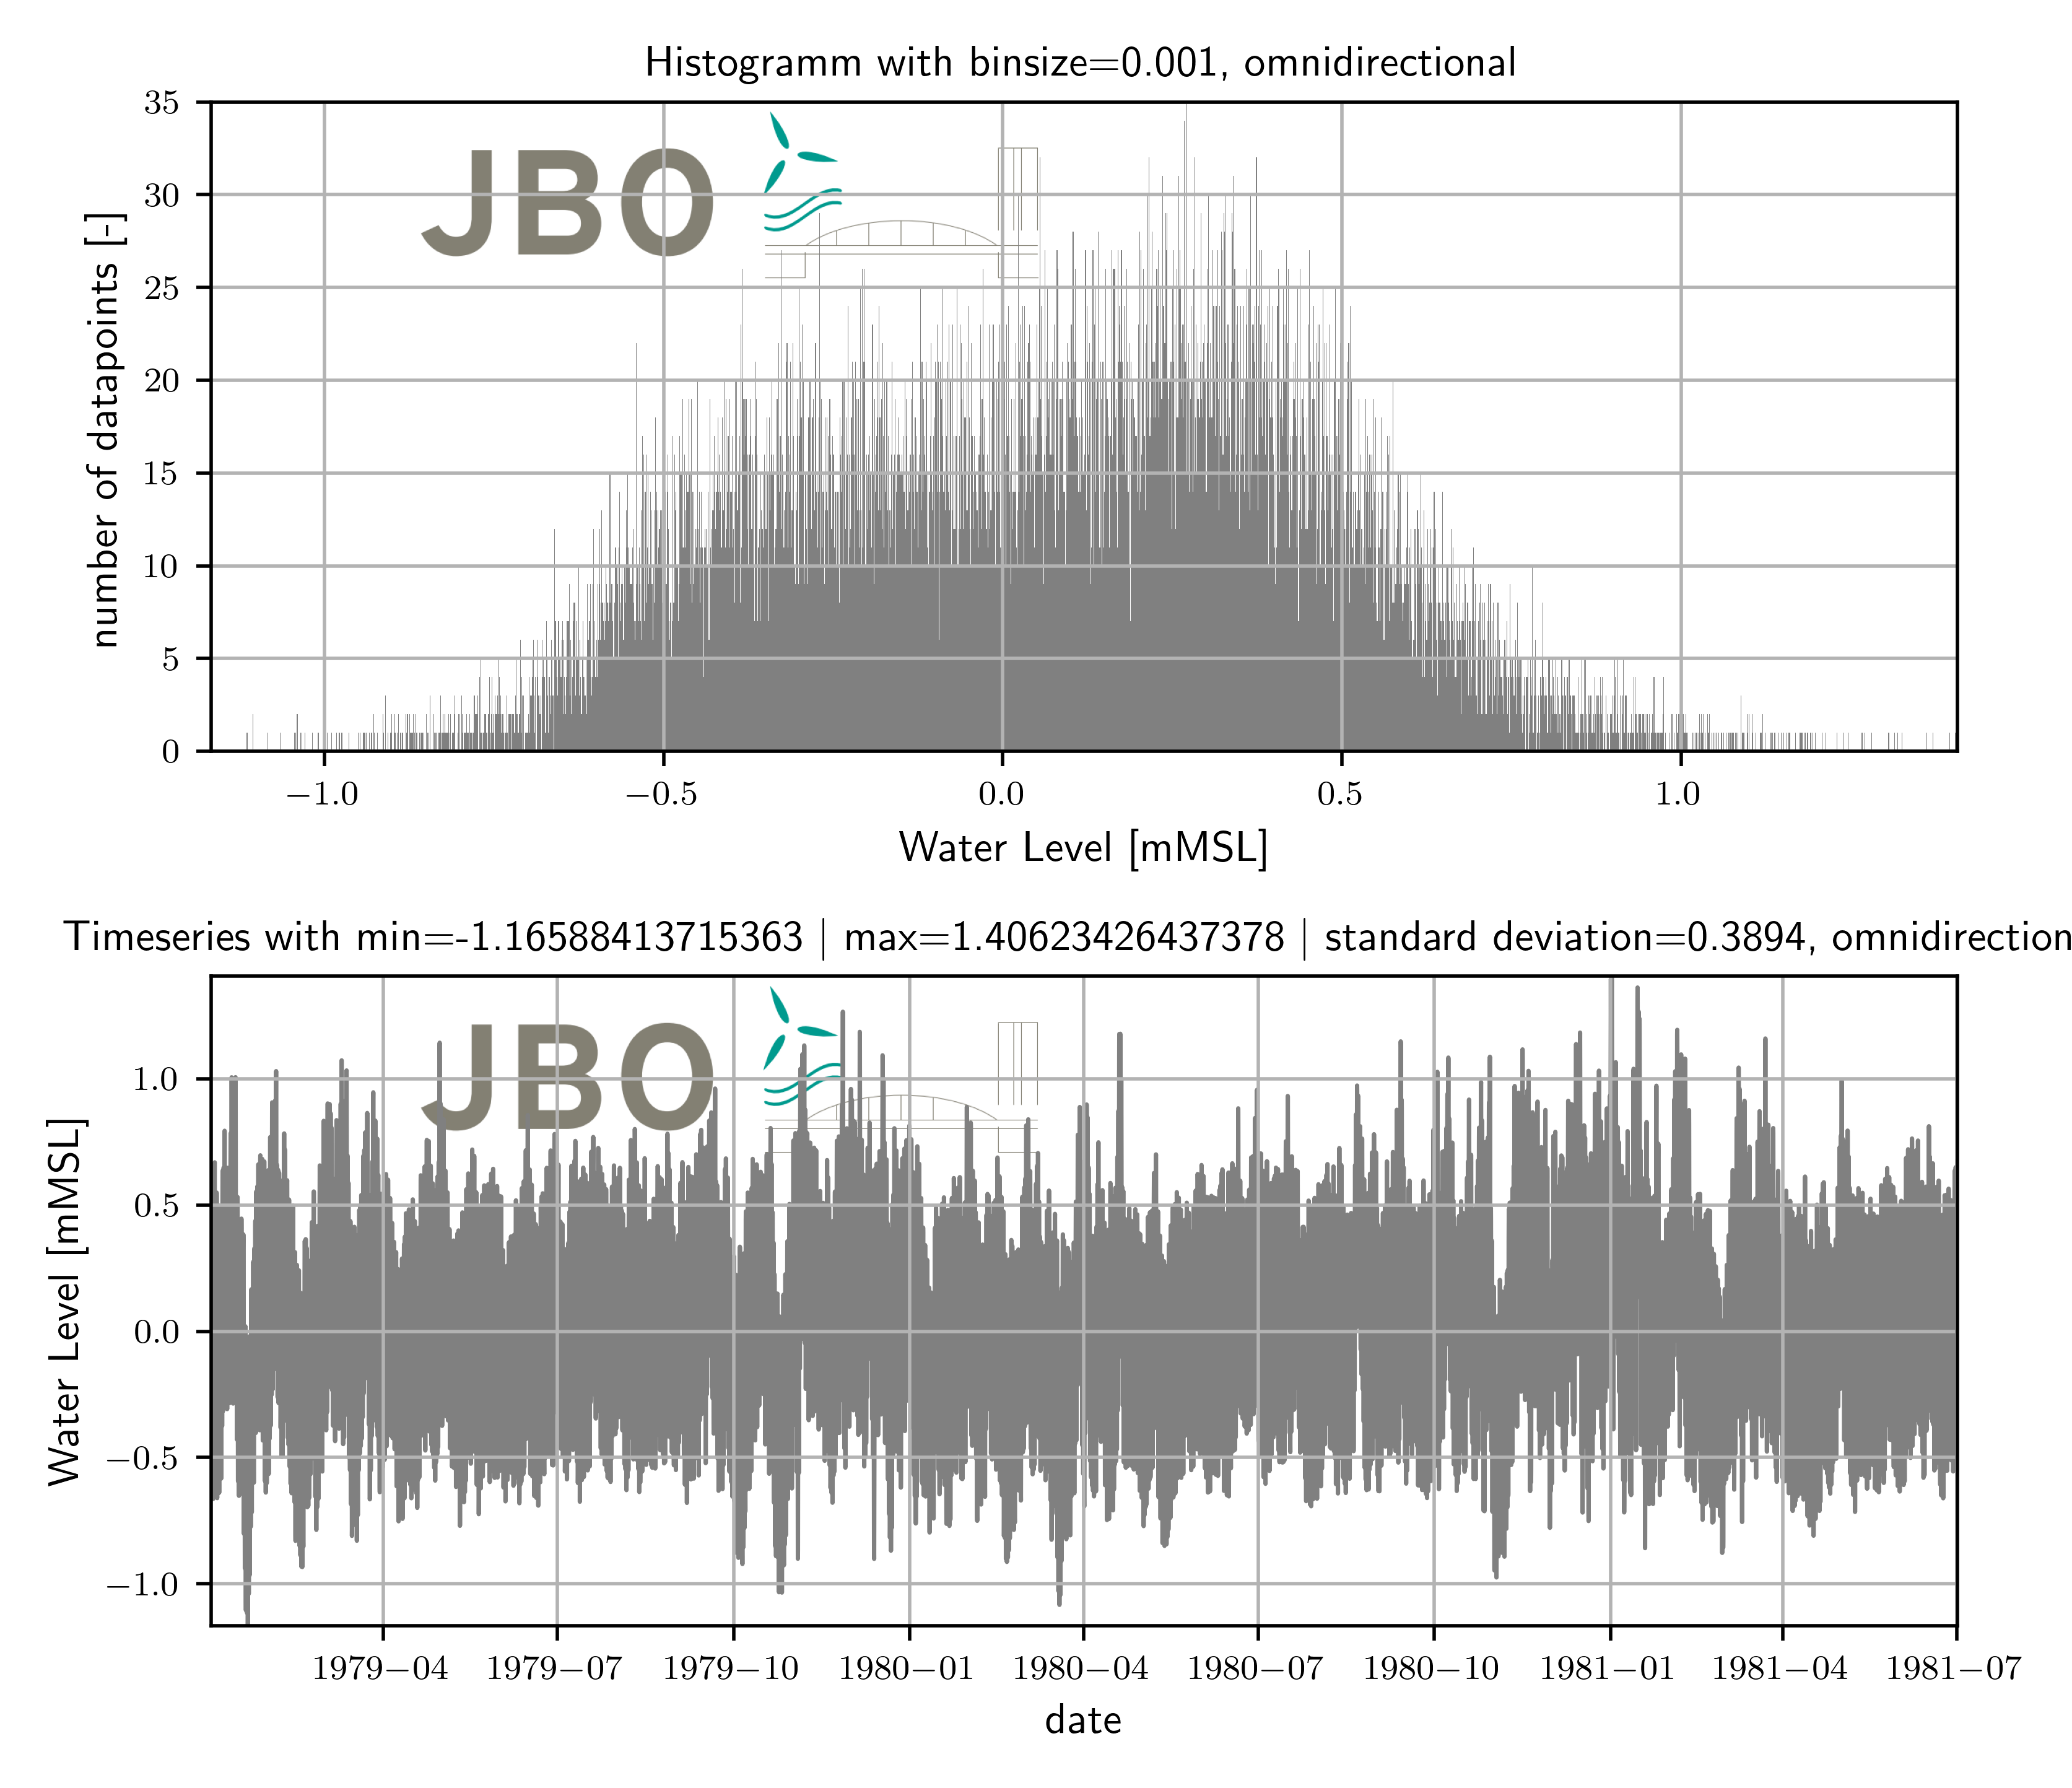
\includegraphics[width=1.0\textwidth]{C:/Users/aaron.lange/Desktop/Projekte/Hindcast_Tool/HindTool/example_output/SensorEval_WL_page_1.png} 
 \caption{ Timeseries and Histogram of Sensor: Water Level [mMSL] } 
 \label{fig: SensorEval_WL_page_1 } 
\end{figure}
 \clearpage
\subsubsection{Sensor: Water Level, Tide [mMSL]} 
\begin{figure}[H] 
 \centering 
 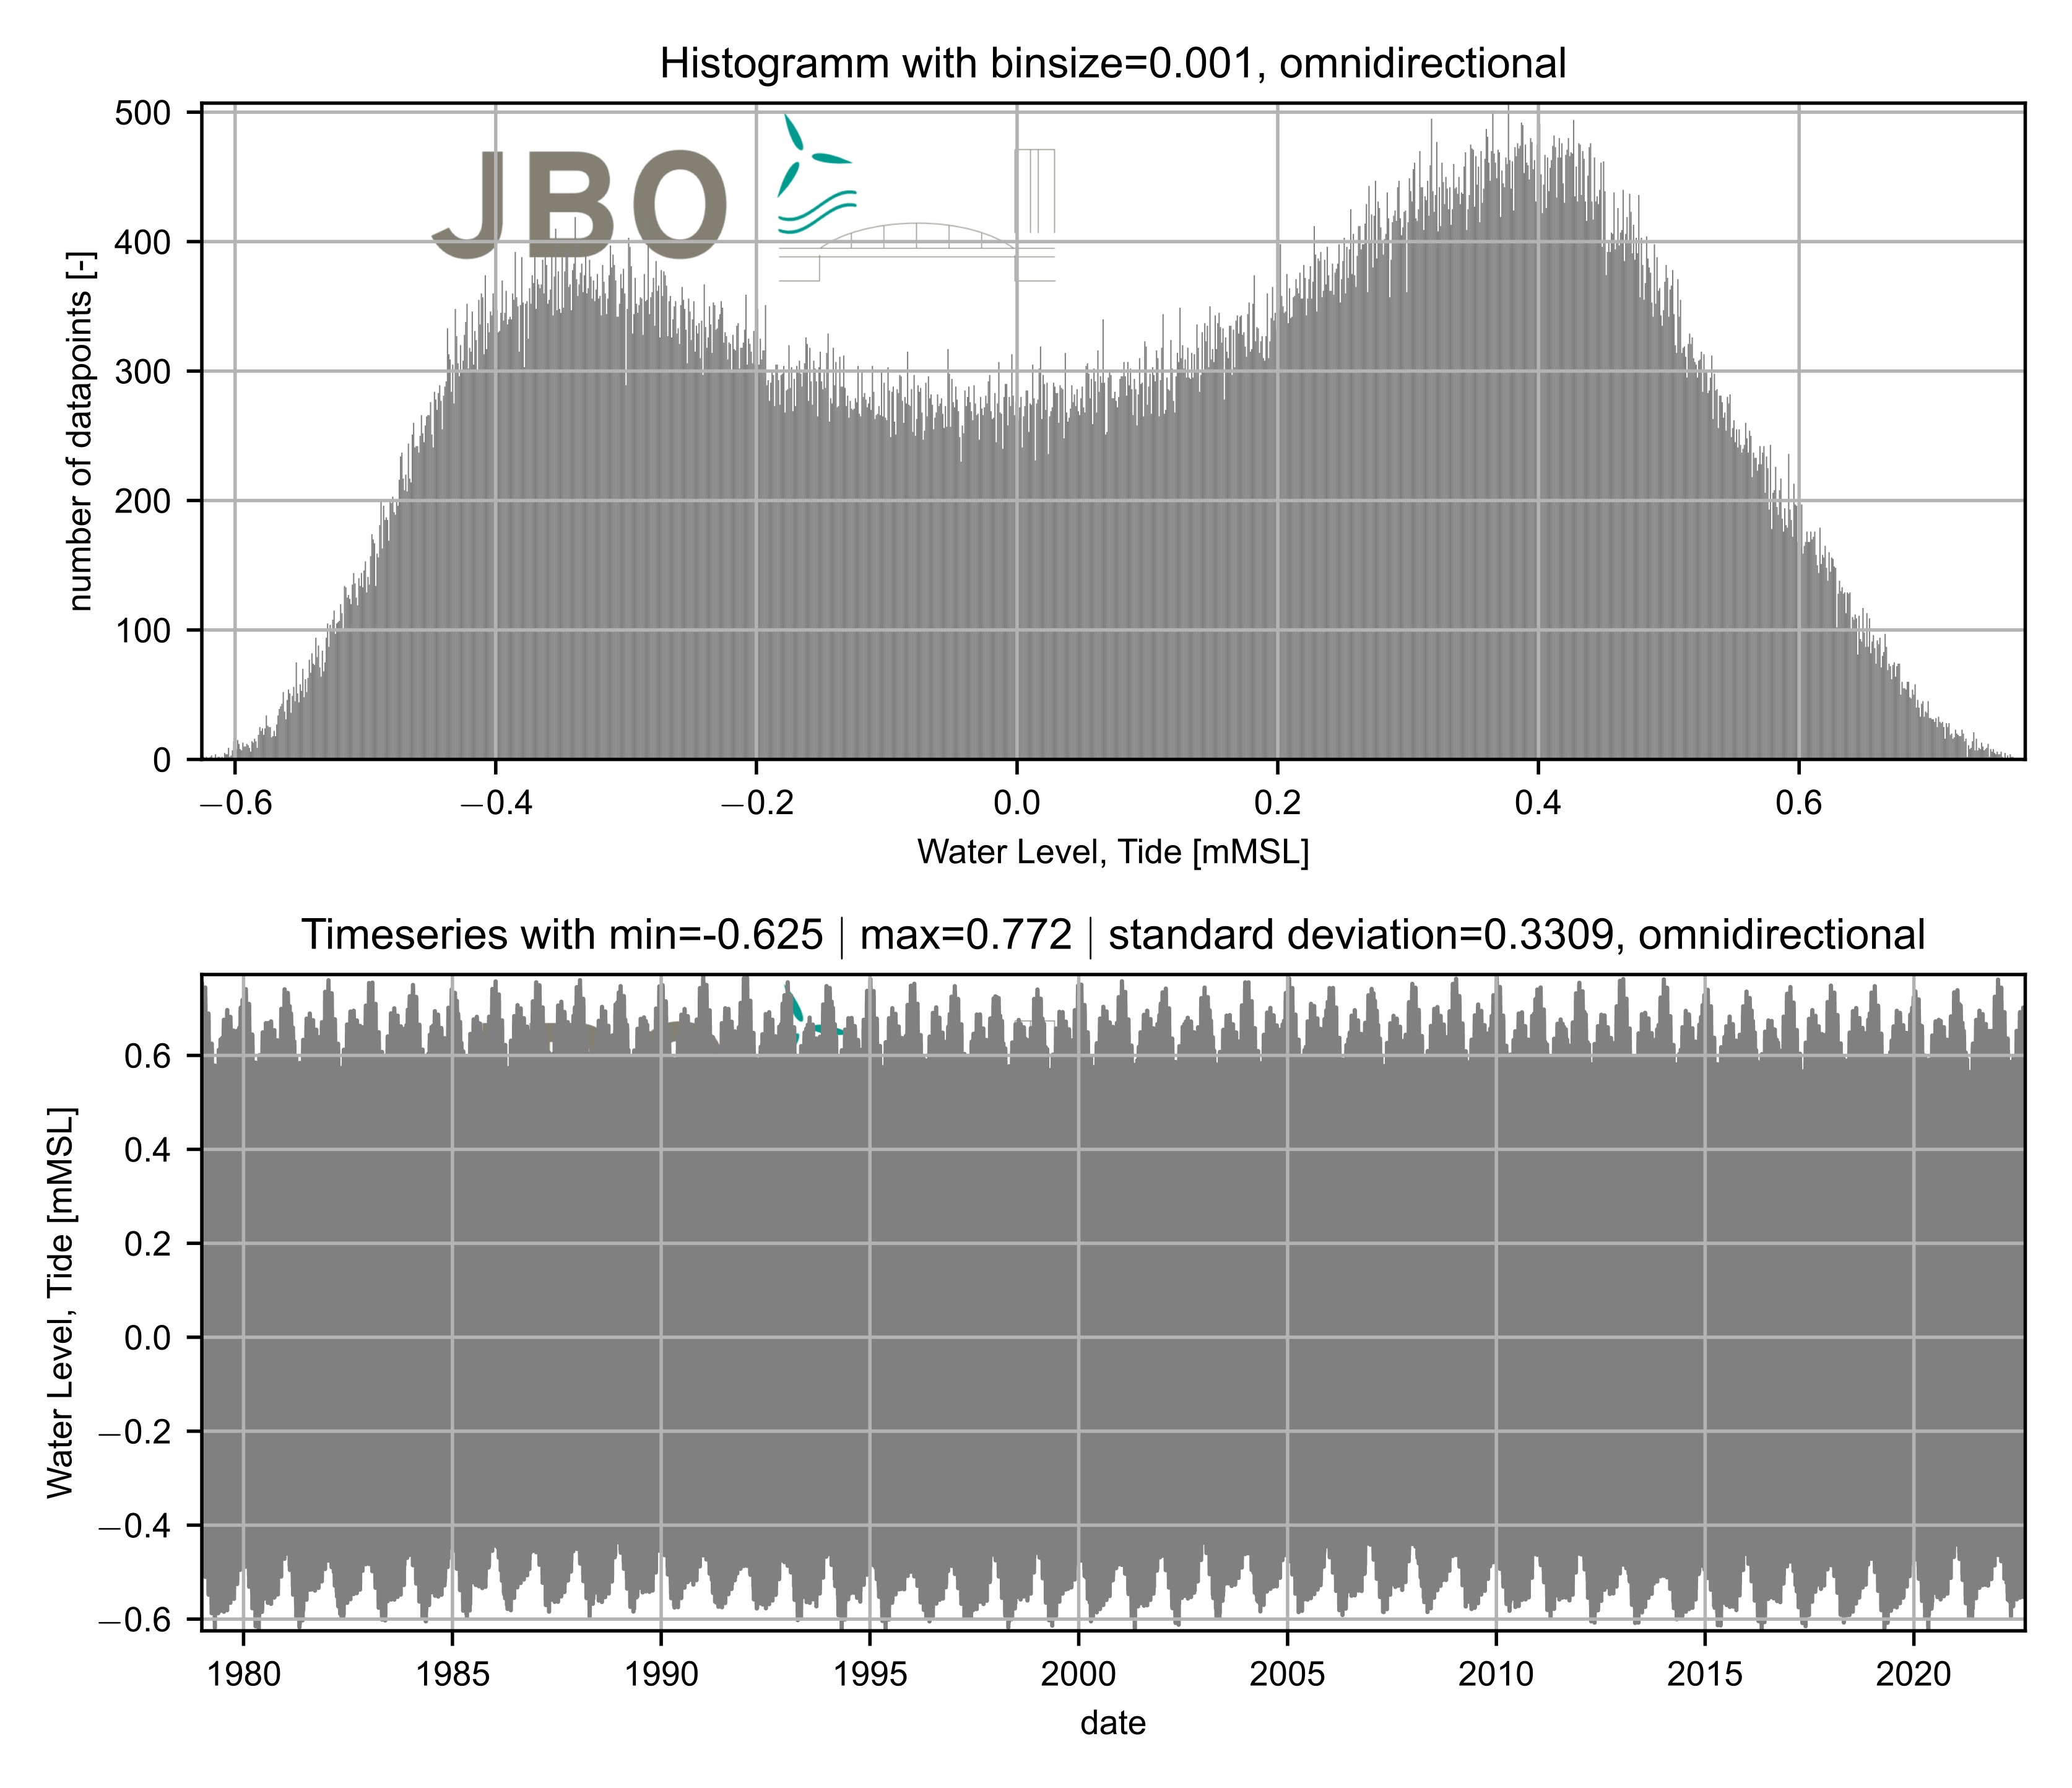
\includegraphics[width=1.0\textwidth]{C:/Users/aaron.lange/Desktop/Projekte/Hindcast_Tool/HindTool/example_output/SensorEval_WL_tide_page_1.png} 
 \caption{ Timeseries and Histogram of Sensor: Water Level, Tide [mMSL] } 
 \label{fig: SensorEval_WL_tide_page_1 } 
\end{figure}
 \clearpage
\subsubsection{Sensor: Current Speed Surface [m/s]} 
\begin{figure}[H] 
 \centering 
 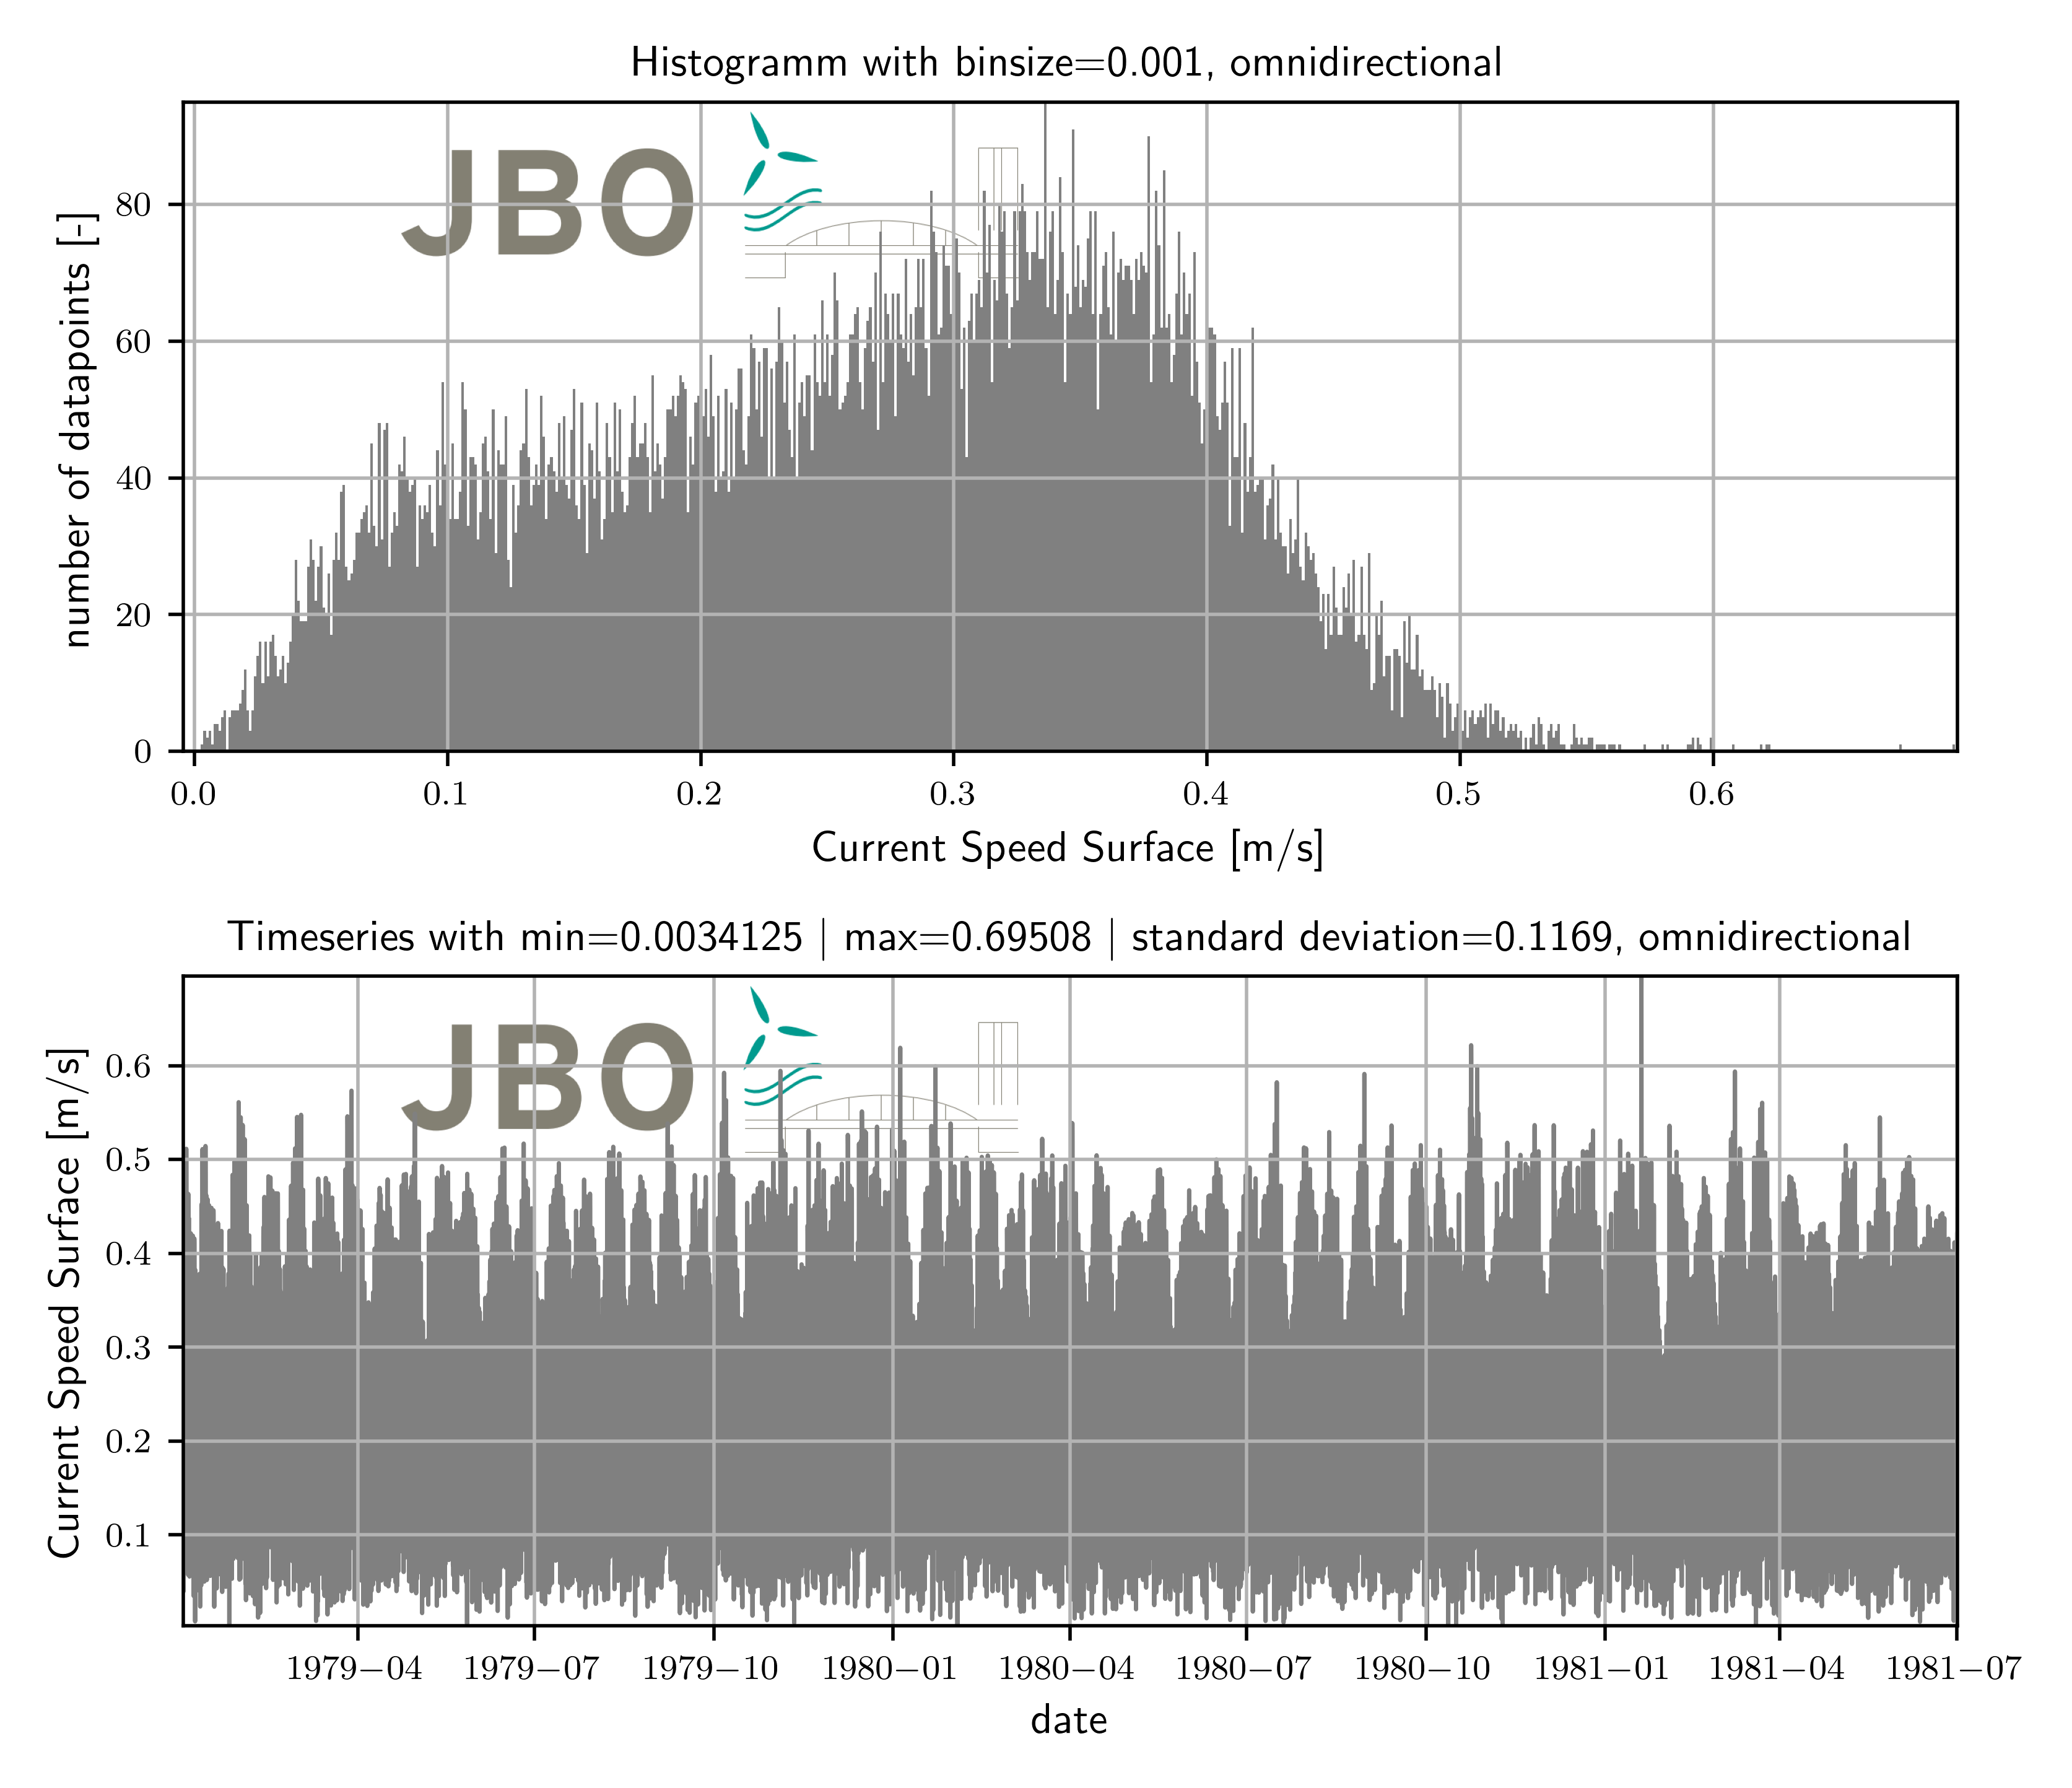
\includegraphics[width=1.0\textwidth]{C:/Users/aaron.lange/Desktop/Projekte/Hindcast_Tool/HindTool/example_output/SensorEval_v_curr_page_1.png} 
 \caption{ Timeseries and Histogram of Sensor: Current Speed Surface [m/s] } 
 \label{fig: SensorEval_v_curr_page_1 } 
\end{figure}
 \clearpage

\subsection{Sensor directional analysis}
Relevant directional sensor evaluations are shown below. 

\subsubsection{Wind direction and wind speed occurrence}

\begin{figure}[H] 
 \centering 
 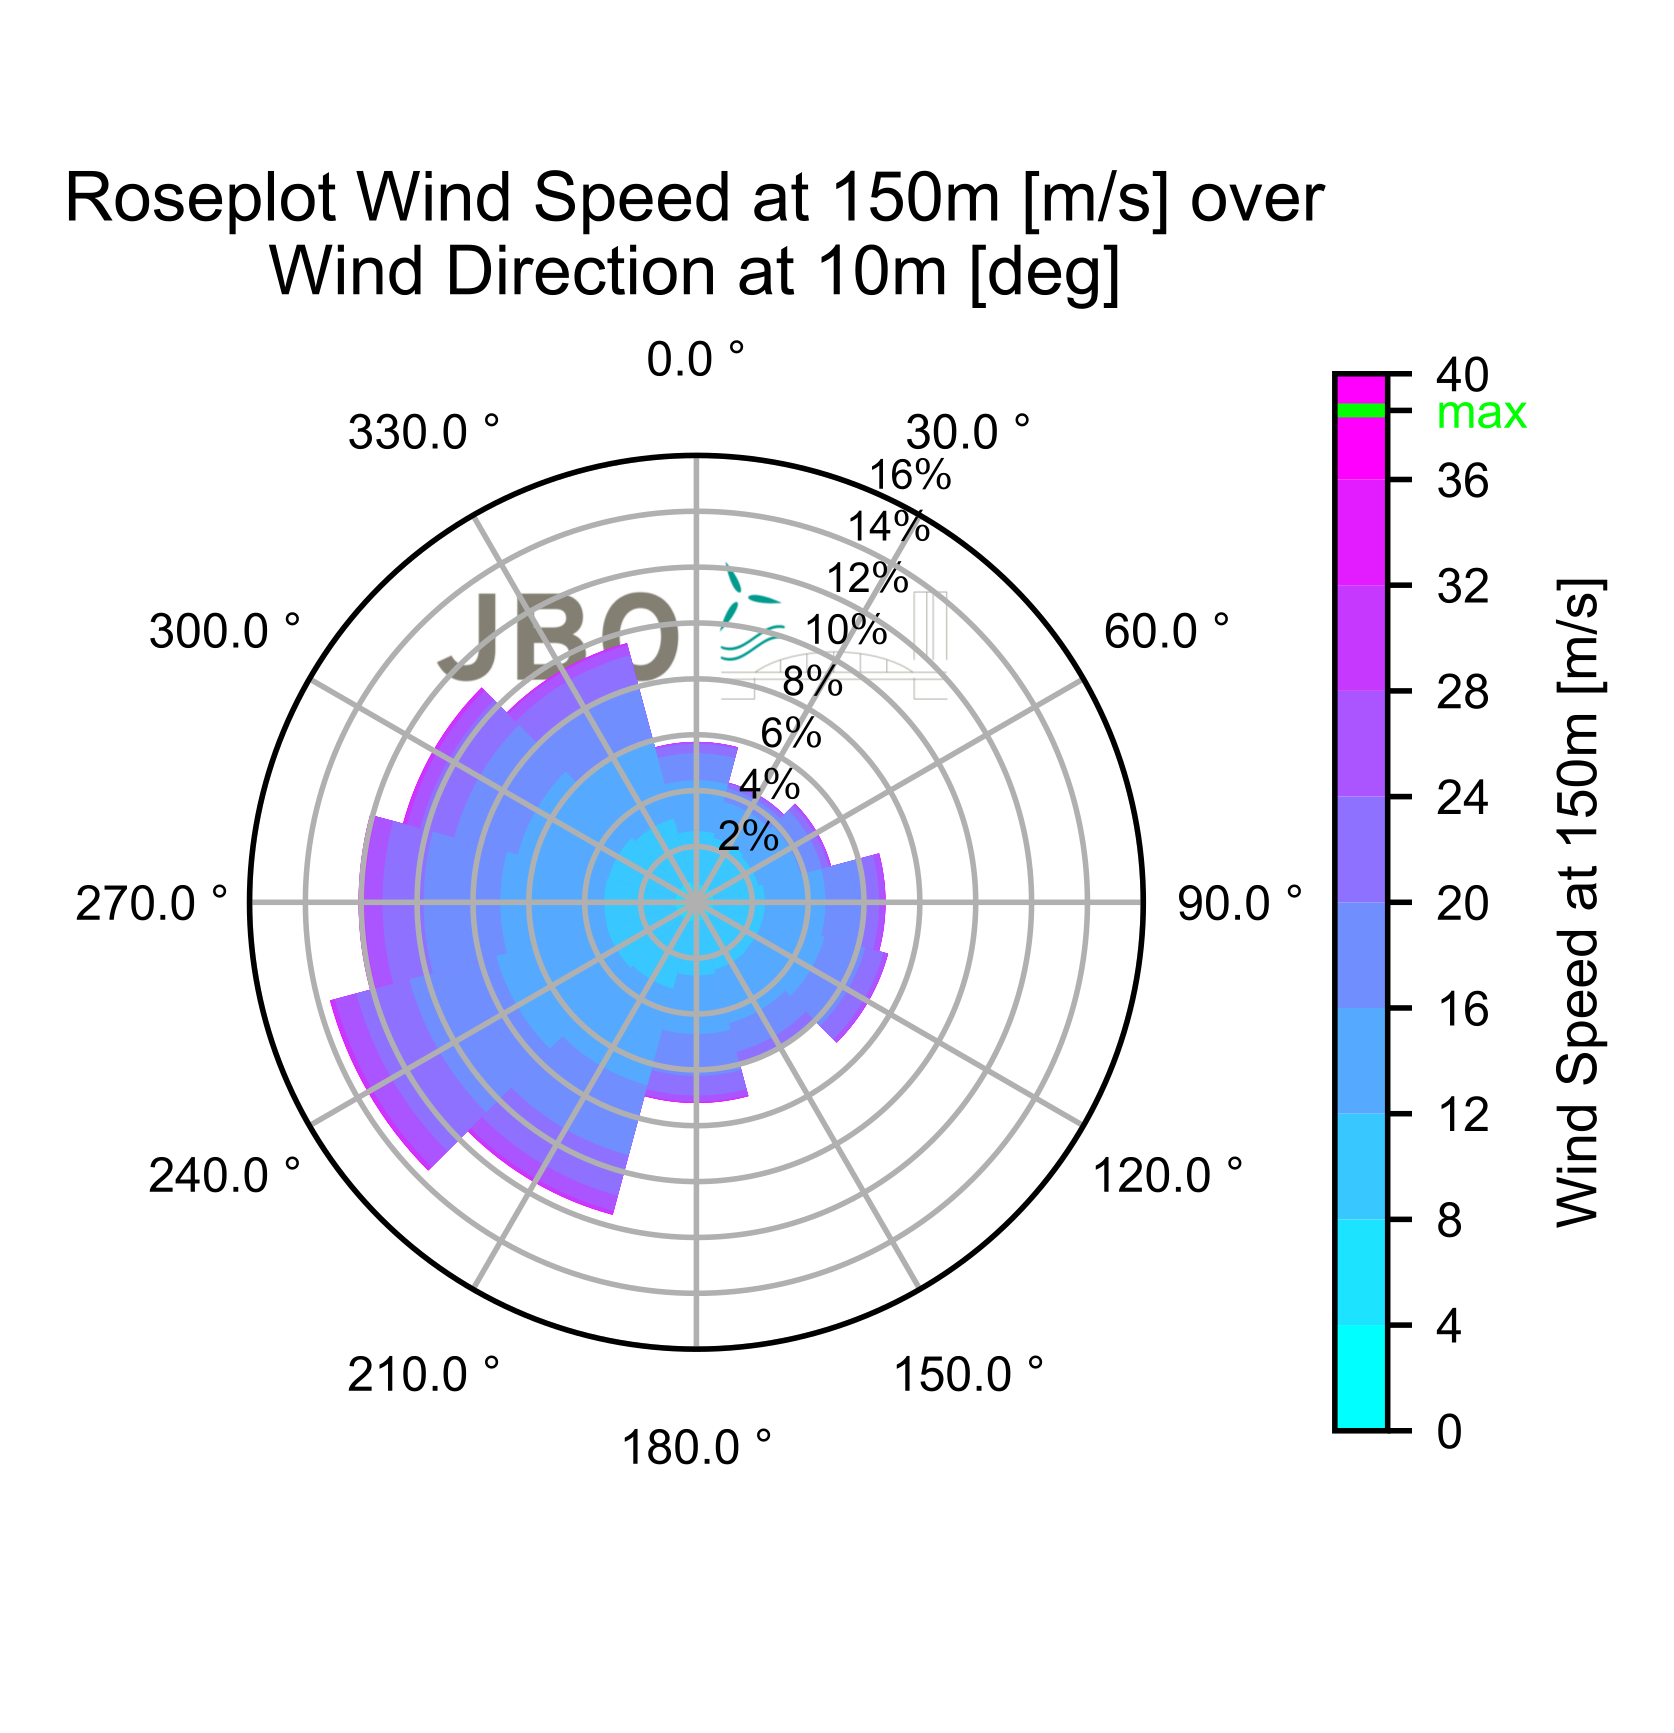
\includegraphics[width=1.0\textwidth]{C:/Users/aaron.lange/Desktop/Projekte/Hindcast_Tool/HindTool/example_output/Roseplots_wind_page_1.png} 
 \caption{ Roseplots-wind-page-1 } 
 \label{fig: Roseplots_wind_page_1 } 
\end{figure}

\subsubsection{Wave direction - Wind Sea}

\begin{figure}[H] 
 \centering 
 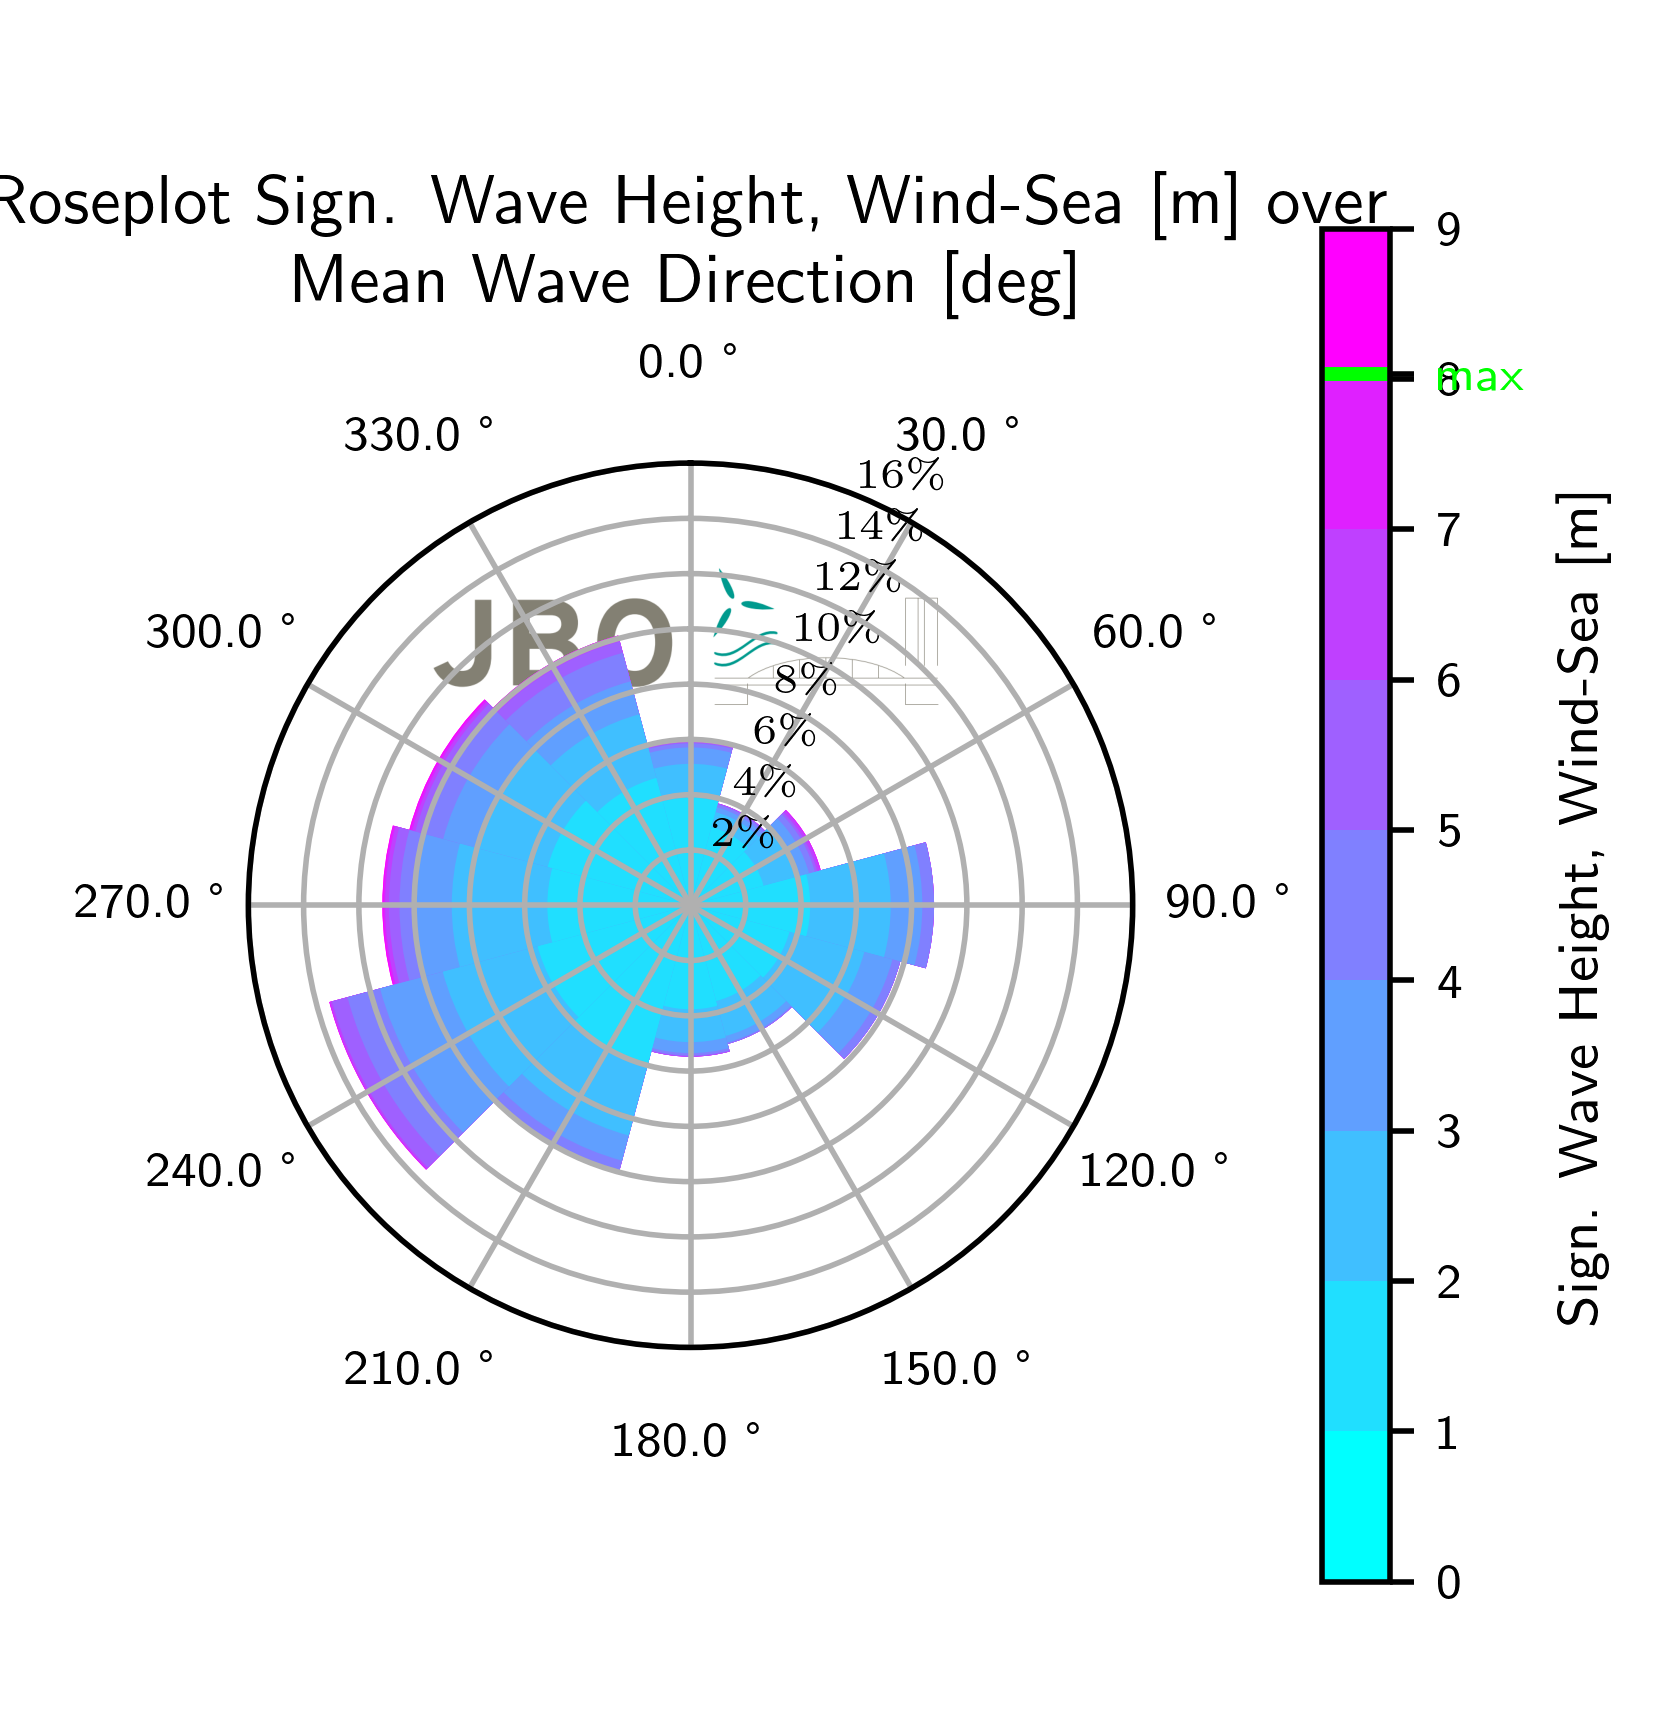
\includegraphics[width=1.0\textwidth]{C:/Users/aaron.lange/Desktop/Projekte/Hindcast_Tool/HindTool/example_output/Roseplots_wind_sea_page_1.png} 
 \caption{ Roseplots-wind-sea-page-1 } 
 \label{fig: Roseplots_wind_sea_page_1 } 
\end{figure}

\subsubsection{Wavedirection - Swell Sea}

\begin{figure}[H] 
 \centering 
 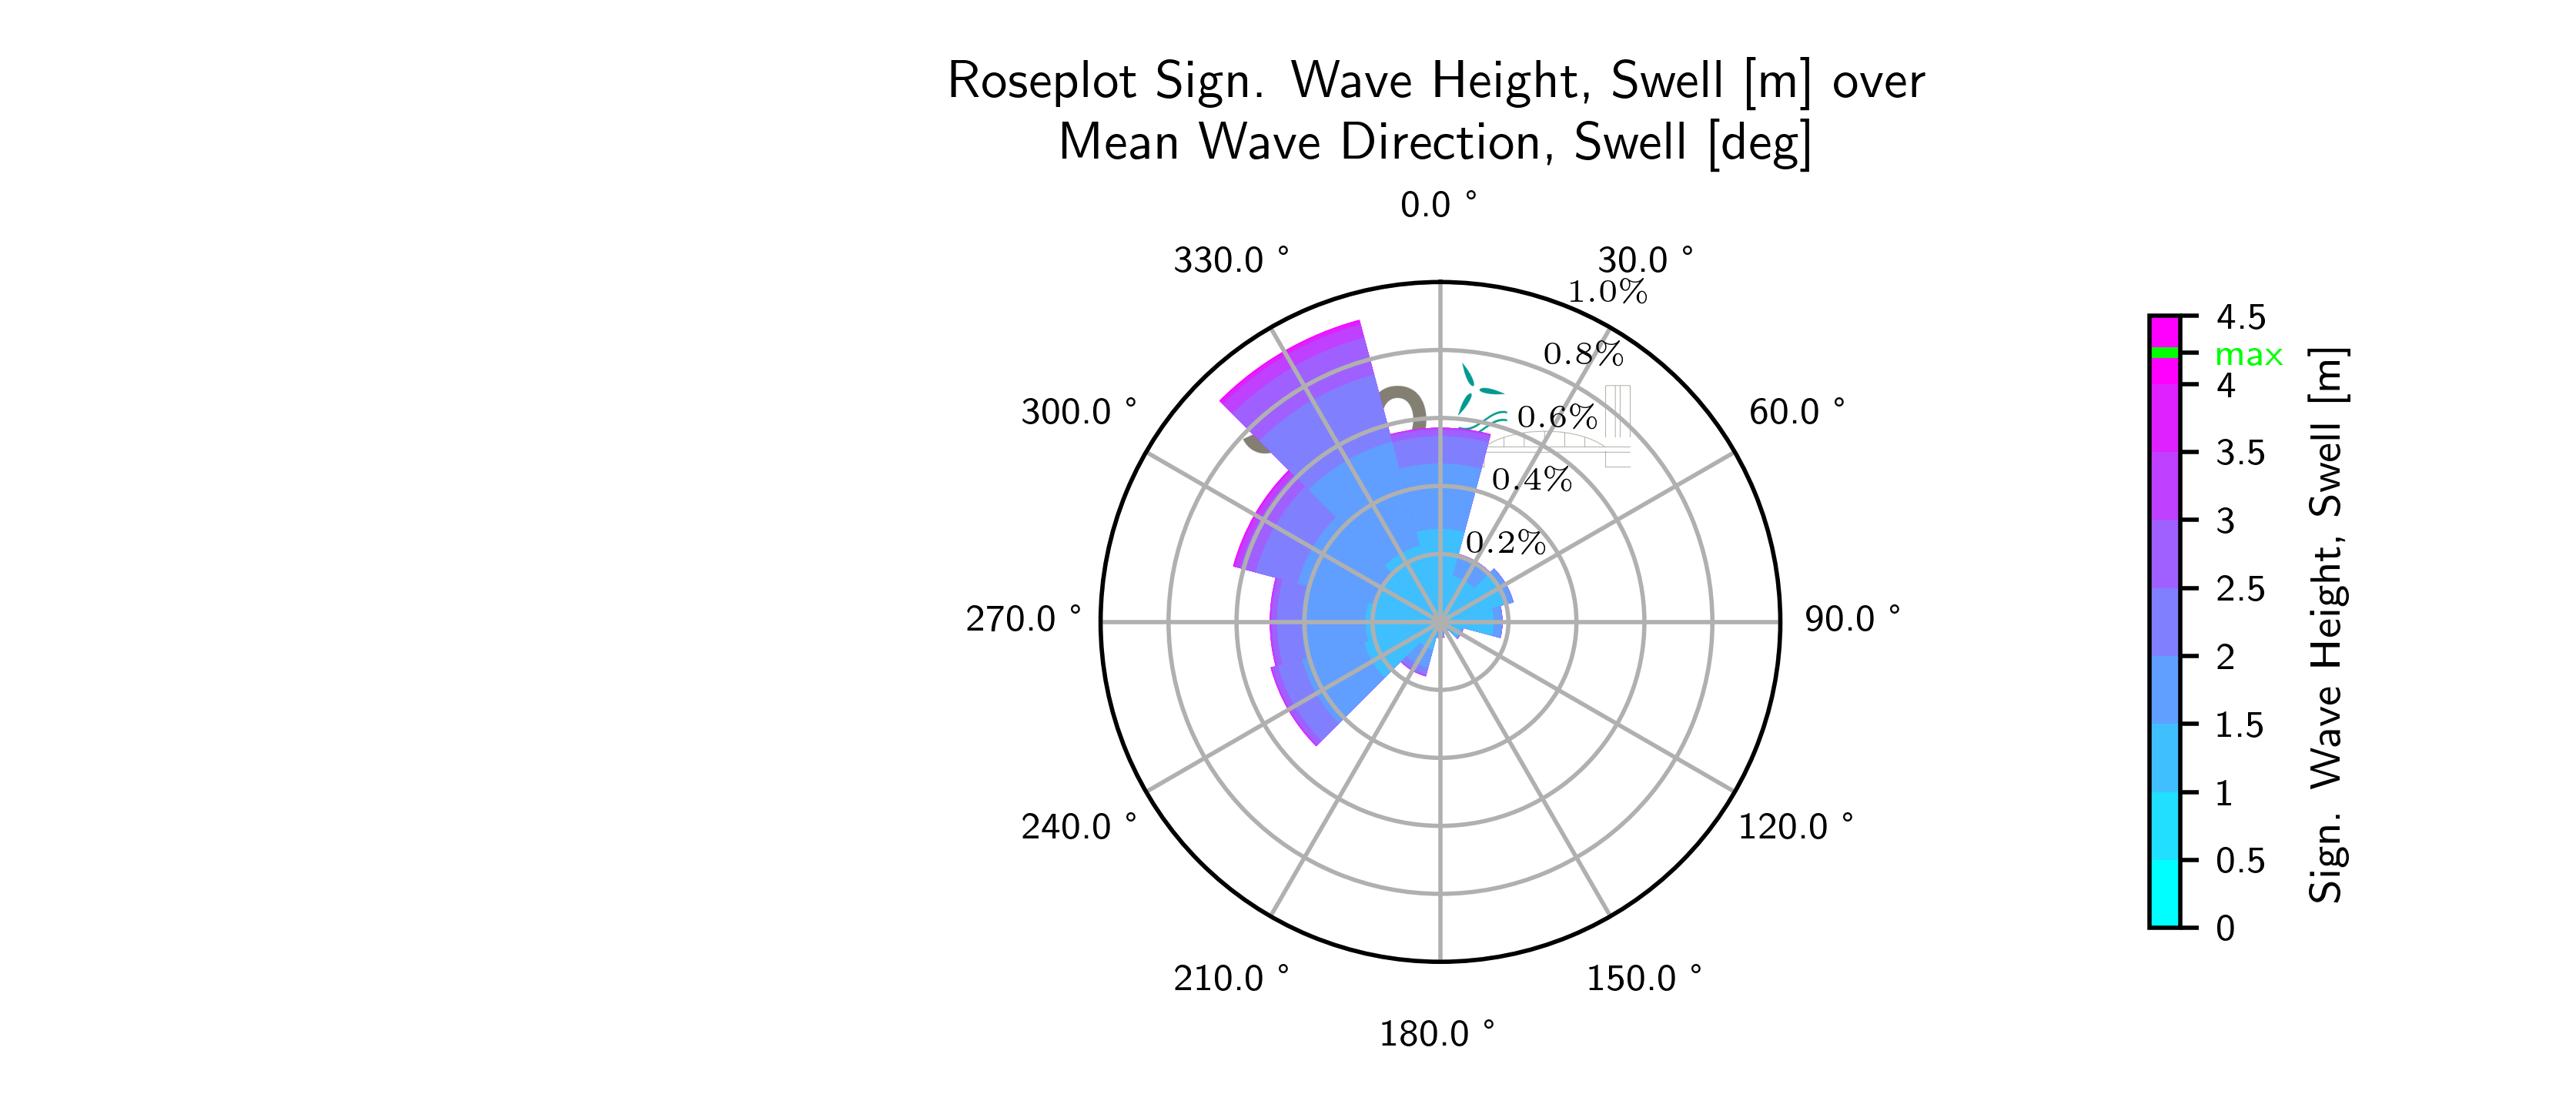
\includegraphics[width=1.0\textwidth]{C:/Users/aaron.lange/Desktop/Projekte/Hindcast_Tool/HindTool/example_output/Roseplots_swell_sea_page_1.png} 
 \caption{ Roseplots-swell-sea-page-1 } 
 \label{fig: Roseplots_swell_sea_page_1 } 
\end{figure}

\subsubsection{Wind - Wave Misalignment}

The occurrence probability of the wind direction and wave direction is considered for normal sea state condition. The misalignment of wind and wave direction, based on the wind direction, is illustrated below. 

\begin{figure}[H] 
 \centering 
 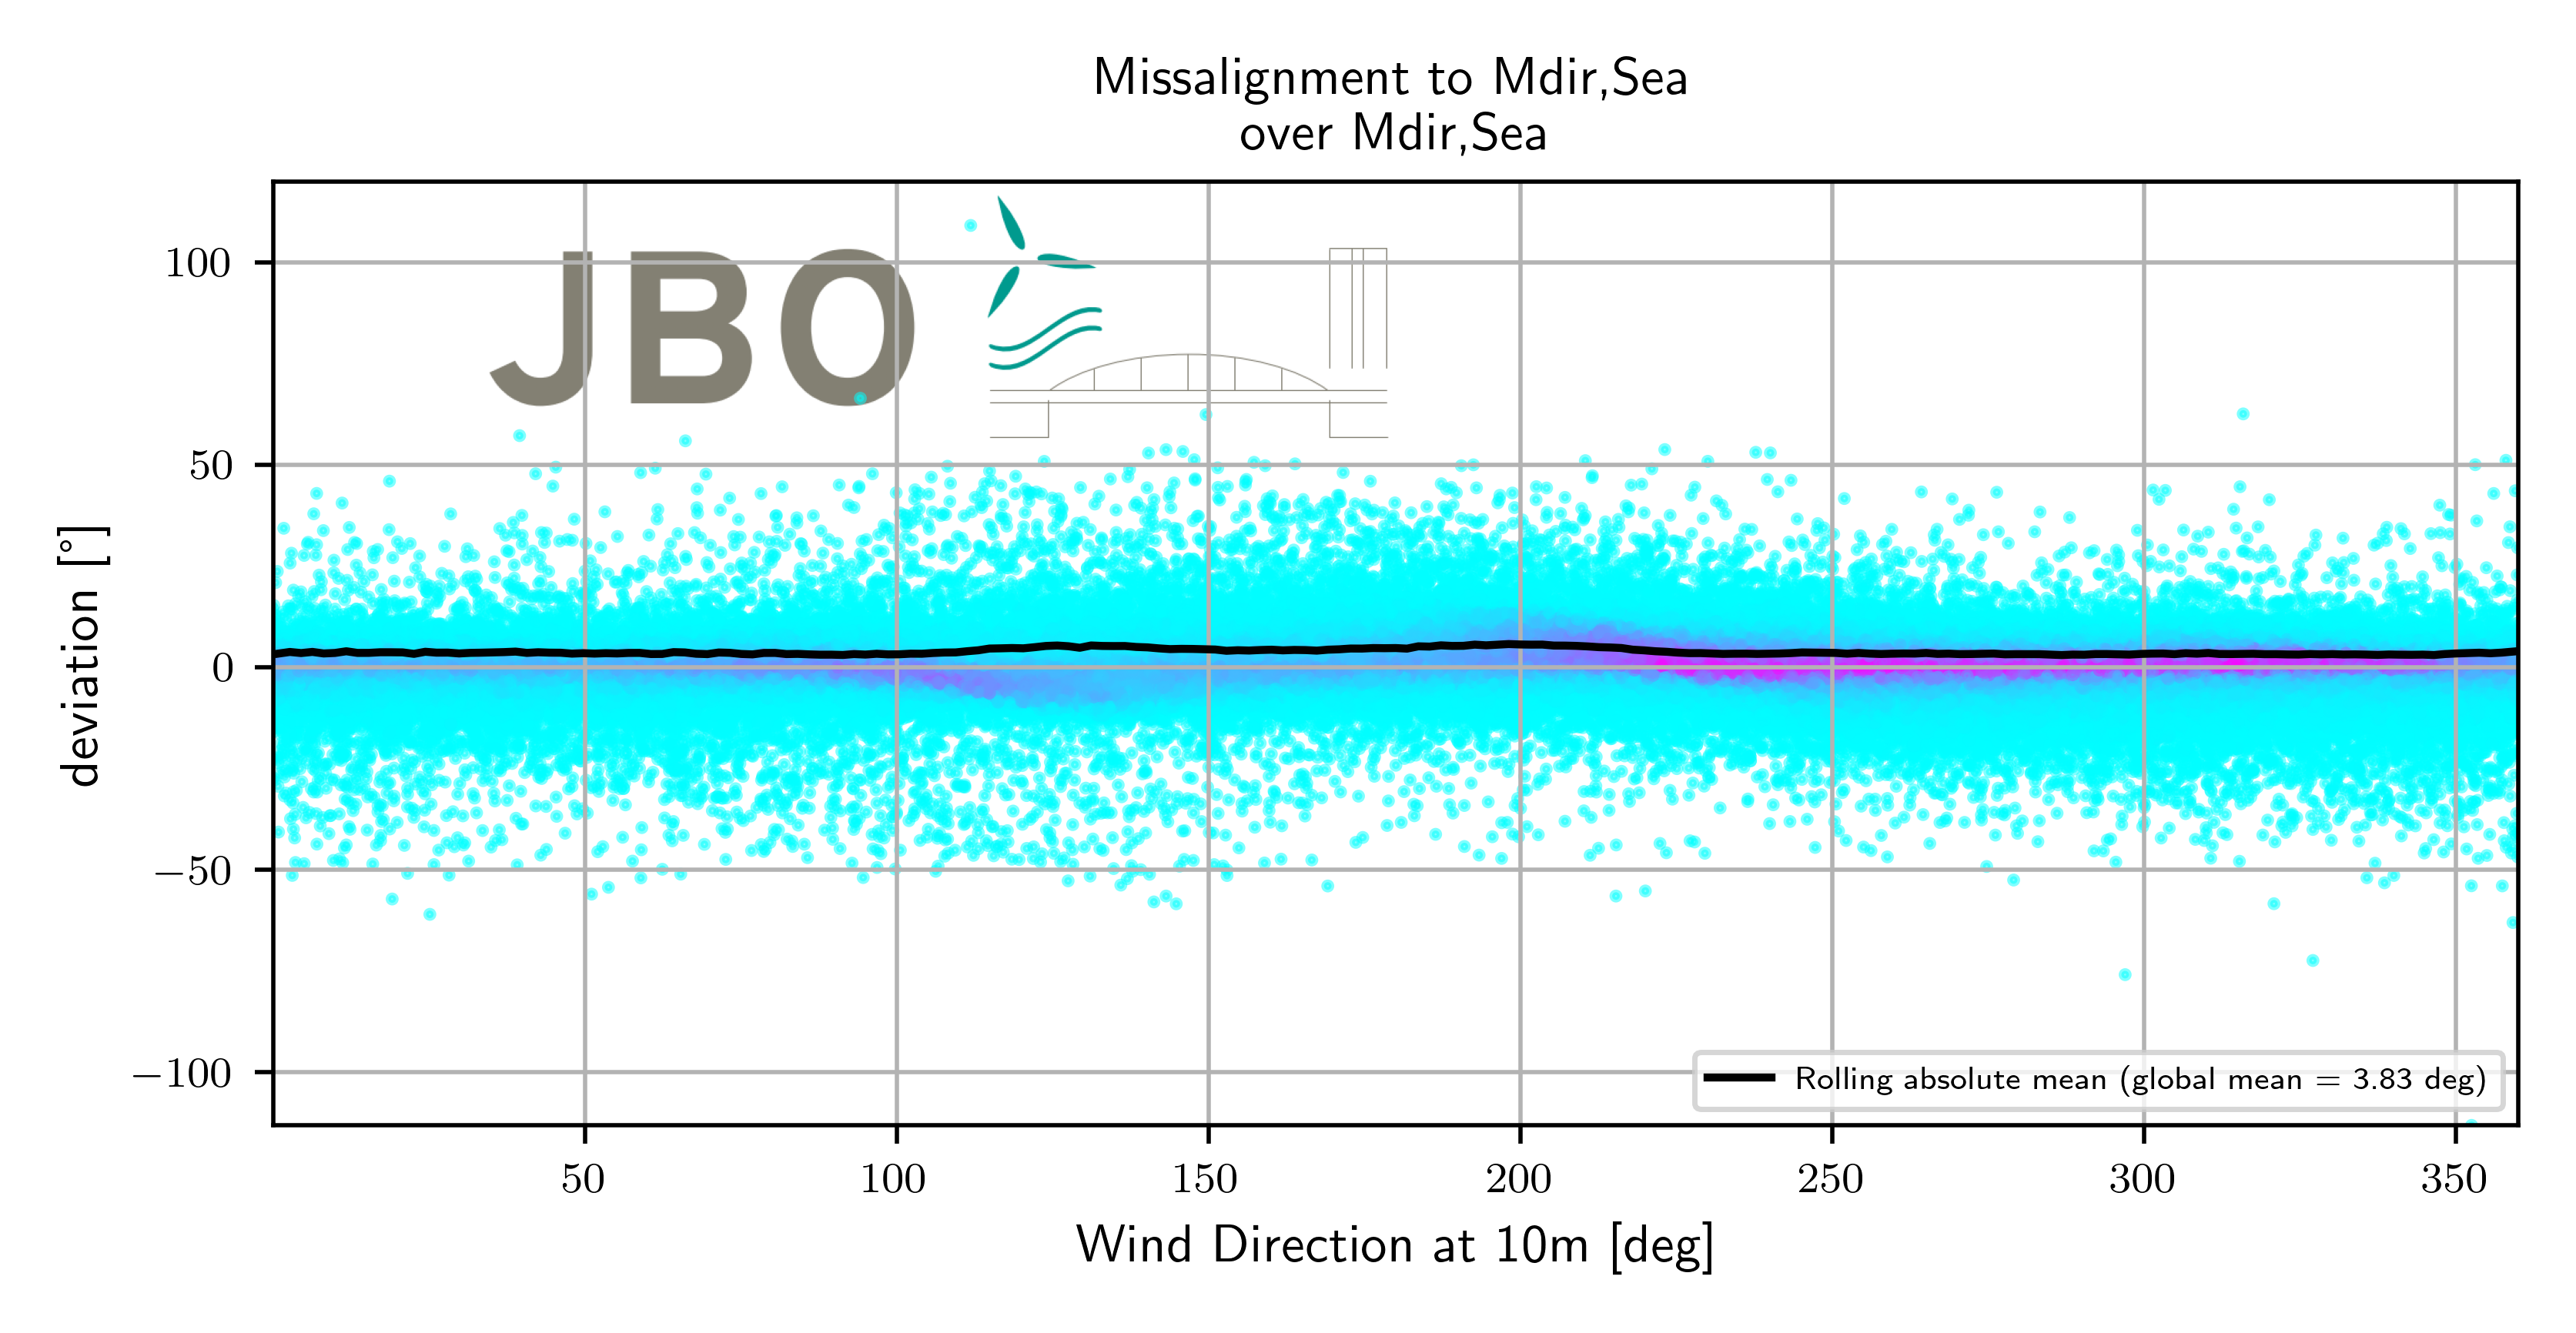
\includegraphics[width=1.0\textwidth]{C:/Users/aaron.lange/Desktop/Projekte/Hindcast_Tool/HindTool/example_output/angle_deviation_scatter_page_1.png} 
 \caption{ angle-deviation-scatter-page-1 } 
 \label{fig: angle_deviation_scatter_page_1 } 
\end{figure}

For the assignment of probabilities to the load situations in the design load case table, the data set is evaluated for each wind speed bin (delta = 1 m/s), wind direction and wave direction, both with a sector width of 30° (see Appendix). 


\clearpage
\subsubsection{Current direction and current speed occurrence}

\begin{figure}[H] 
 \centering 
 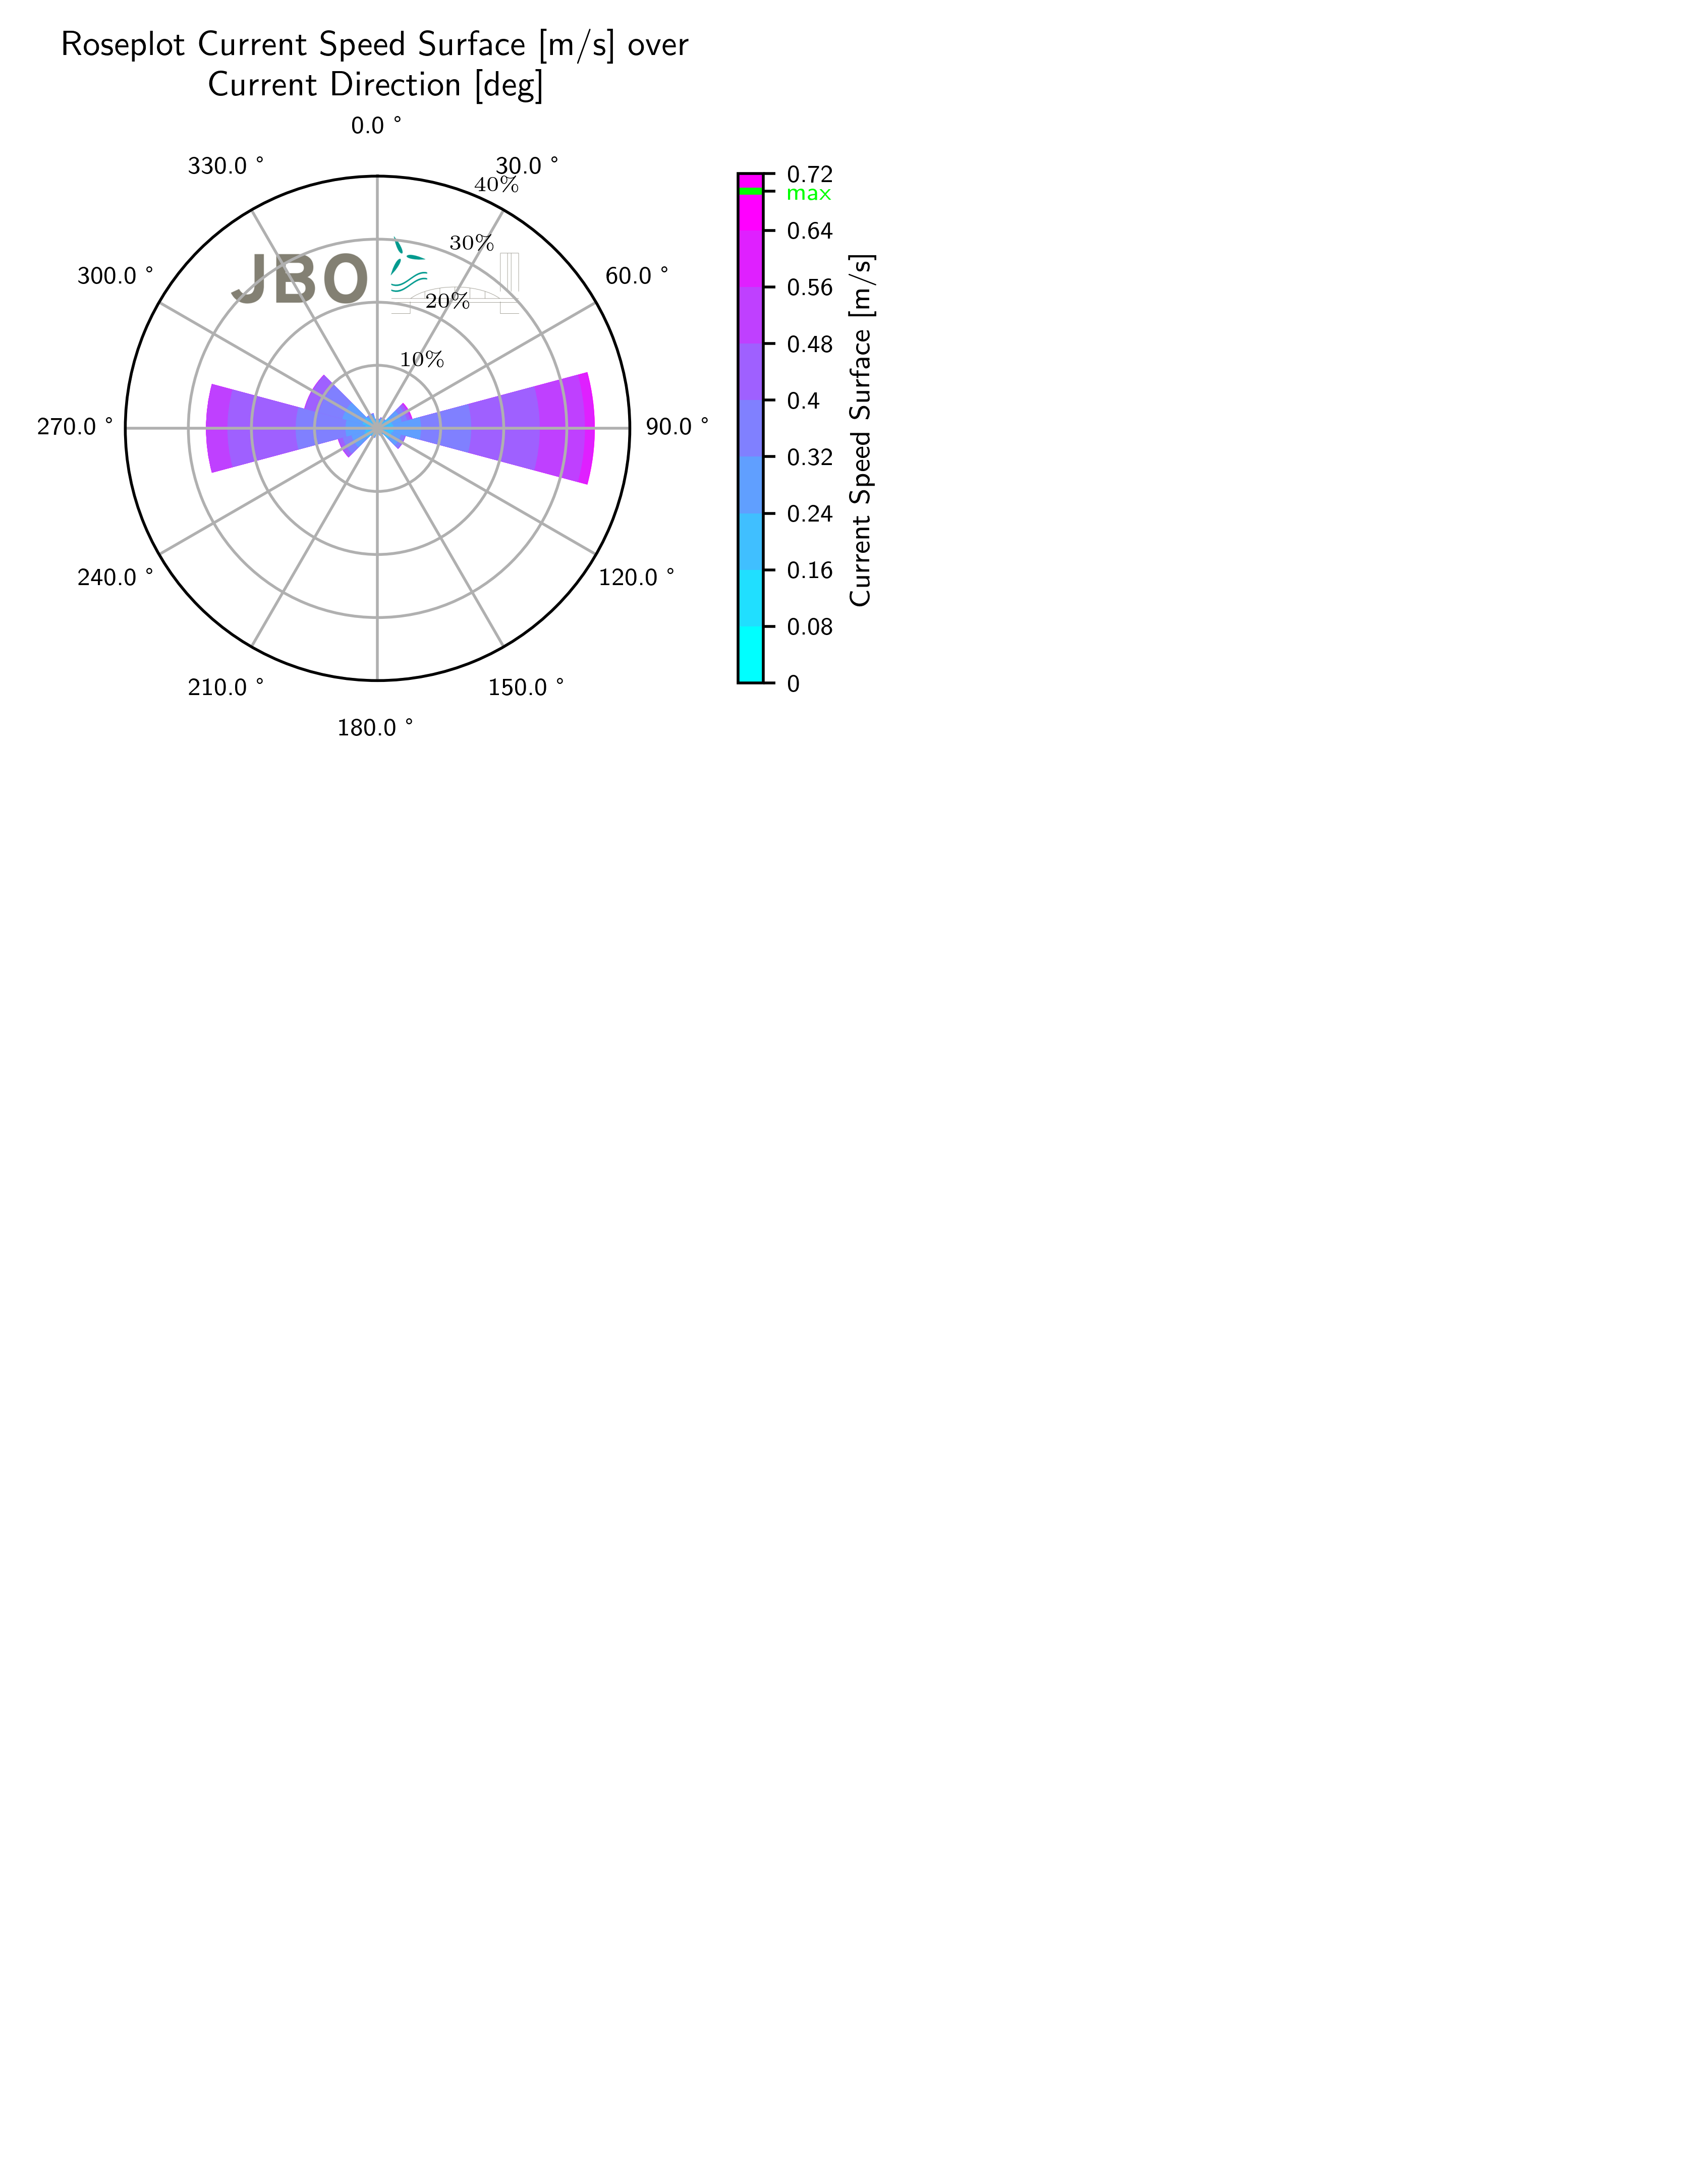
\includegraphics[width=1.0\textwidth]{C:/Users/aaron.lange/Desktop/Projekte/Hindcast_Tool/HindTool/example_output/Roseplots_currents_page_1.png} 
 \caption{ Roseplots-currents-page-1 } 
 \label{fig: Roseplots_currents_page_1 } 
\end{figure}